\chapter{Learning Photometric Stereo} 
\label{ch:psfcn}

\section{Introduction}
\begin{figure}[t]
\centering
    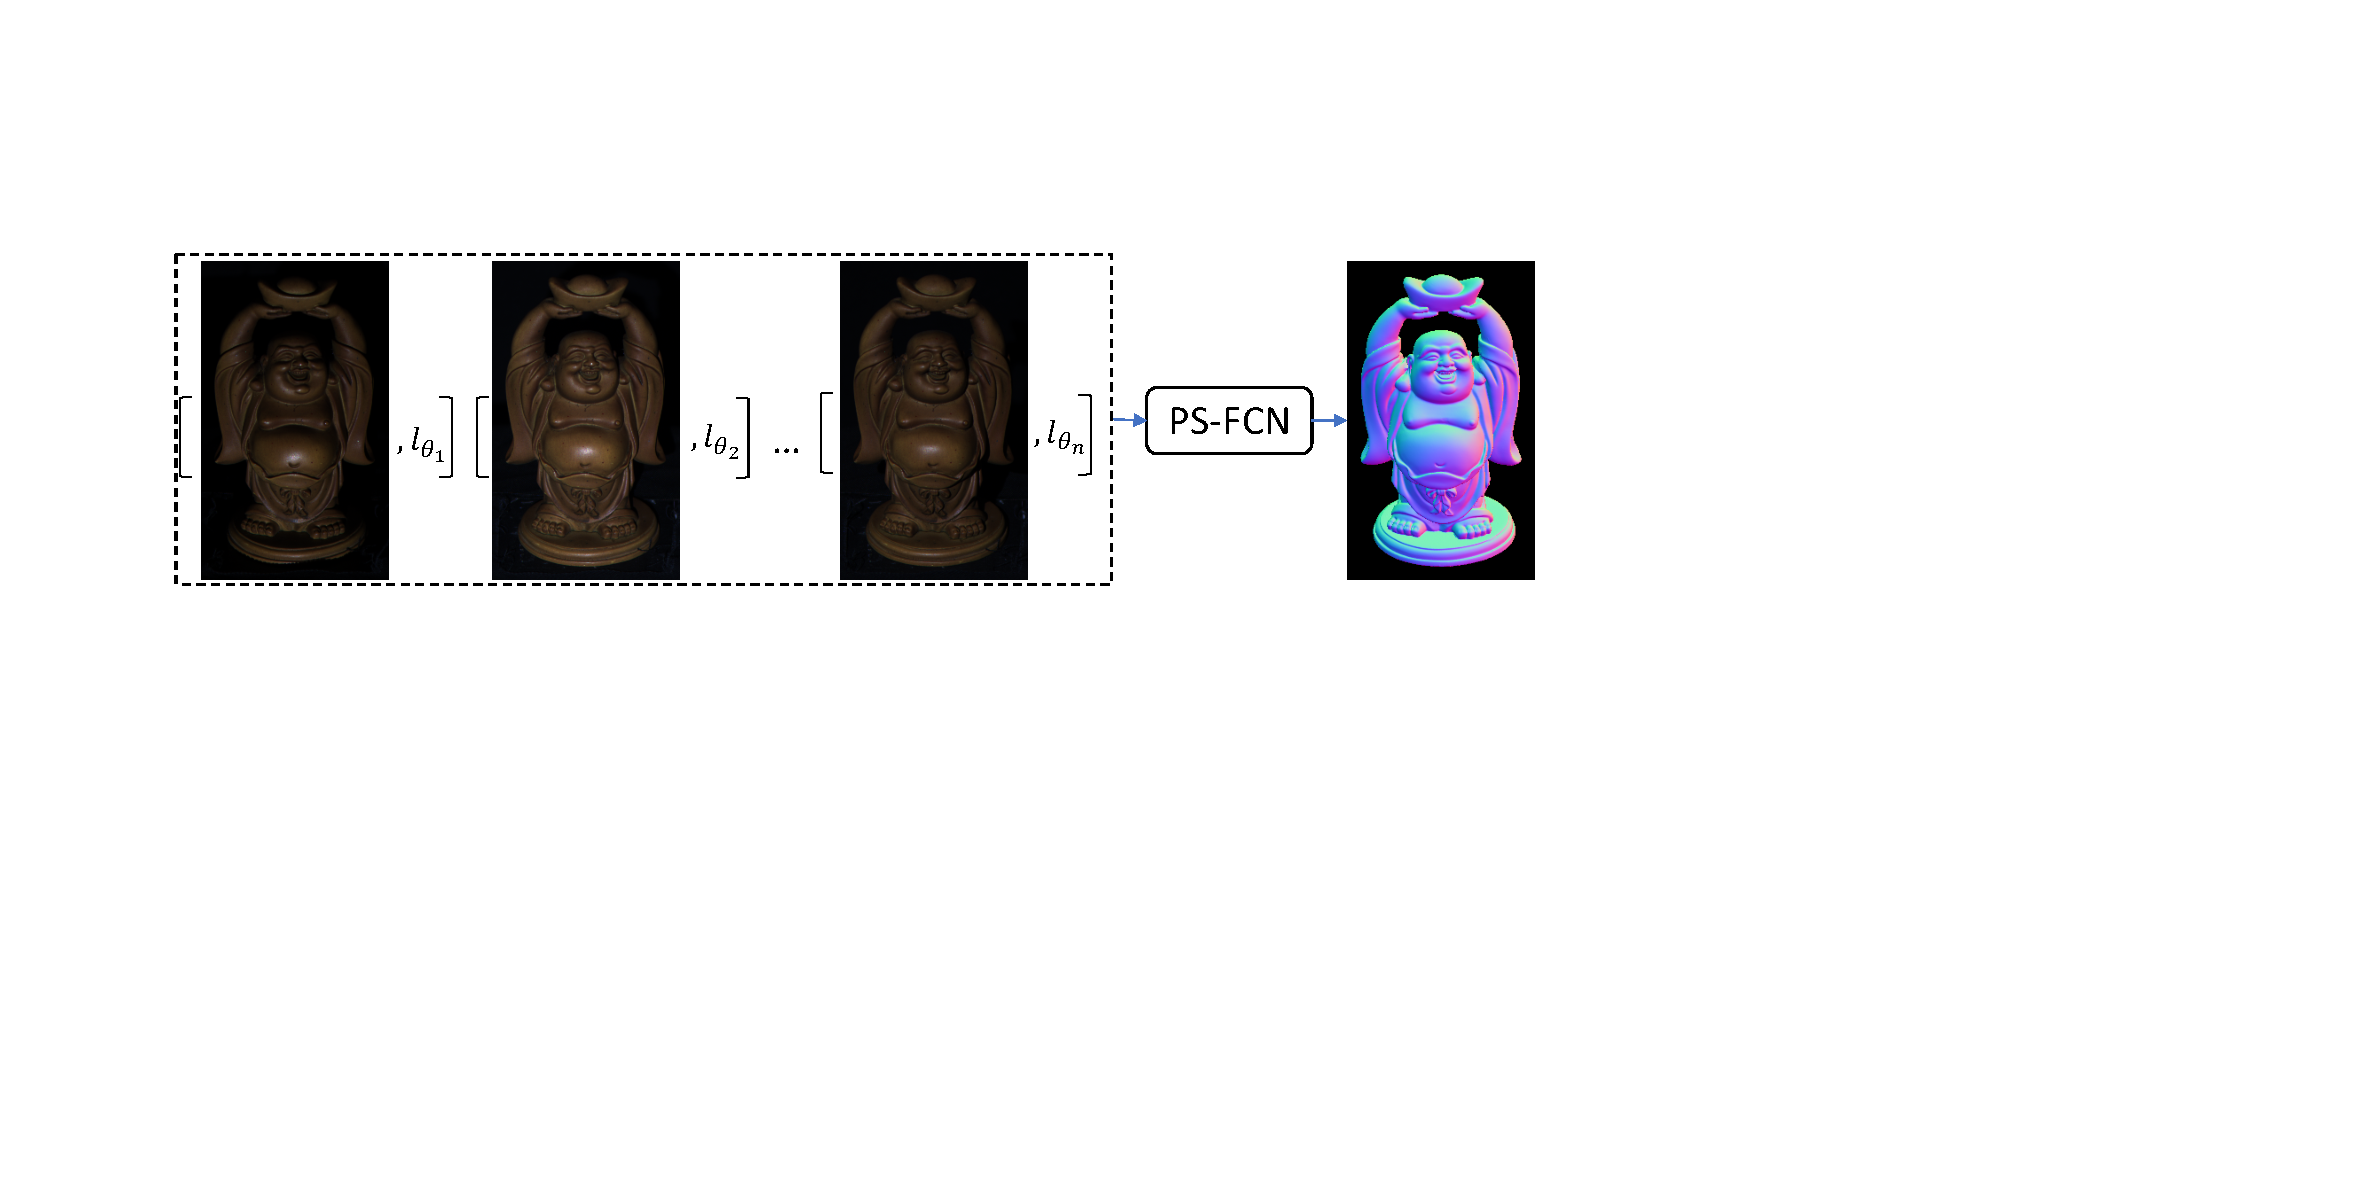
\includegraphics[width=\textwidth]{ch-psfcn/images/Intro/Intro.pdf}
    \caption[Learning photometric stereo]{Given an arbitrary number of images and their associated light directions as input, our model estimates a normal map of the object in a fast feed-forward pass.} \label{fig:Intro}
\end{figure}

Given multiple images of a static object captured under different light directions with a fixed camera, the surface normals of the object can be estimated using photometric stereo techniques. 
Early calibrated photometric stereo methods assumed a simplified reflectance model, such as the ideal Lambertian model~\cite{woodham1980ps,silver1980determining} or analytical reflectance models~\cite{tozza2016direct,chung2008efficient,ruiters2009heightfield}. 
However, most of the real-world objects are non-Lambertian, and a specific analytical model is only valid for a small set of materials. A bidirectional reflectance distribution function (BRDF) is a general form for describing the reflectance property of a surface, but it is difficult to directly use a non-parametric form of BRDFs for photometric stereo. 
Hence, it remains an open and challenging problem to develop a computationally efficient photometric stereo method that can handle materials with diverse BRDFs. 

Recently, with the great success of deep learning in various computer vision tasks, deep learning based methods have been introduced to calibrated photometric stereo to handle surfaces with general and unknown isotropic reflectance~\cite{santo2017deep,ikehata2018cnn,Taniai18}. Instead of explicitly modeling complex surface reflectances, they directly learn the mapping from reflectance observations to surface normals given known light directions. 
However, the method in~\cite{santo2017deep} depends on a pre-defined set of light directions during training and testing. The methods in~\cite{santo2017deep,ikehata2018cnn} estimate the surface normals in a pixel-wise manner, making them not possible to account for the local context information of a surface point (\eg, surface smoothness prior).
Taniai and Maehara~\cite{Taniai18} introduced an optimization framework based on deep neural network, but their method suffers from complex scenes and requires a long processing time. 

In this work, we propose a deep fully convolutional network (FCN)~\cite{long2015fully}, called PS-FCN for calibrated photometric stereo.
PS-FCN takes an arbitrary number of images with their associated light directions as input, and predicts a surface normal map of the scene in a fast feed-forward pass (see~\fref{fig:Intro}).
Compared with previous learning based methods, our method does not depend on a pre-defined set of light directions during training and testing, and can handle multiple images in an order-agnostic manner. 
Moreover, convolutional neural network (CNN) can naturally incorporate information of the observations at neighboring pixels for computing feature maps, allowing our method to take advantage of local context information. 

To simulate real-world complex non-Lambertian surfaces for training PS-FCN, we create two synthetic datasets using shapes from the blobby shape dataset~\cite{johnson2011shape} and the sculpture shape dataset~\cite{wiles2017silnet}, and BRDFs from the MERL BRDF dataset~\cite{matusik2003merl}. After training on synthetic data, we show that PS-FCN can generalize well on real datasets, including the \diligent~\cite{shi2019benchmark}, the \gourd~\cite{alldrin2008p}, and the \lightstage~\cite{einarsson2006relighting}. 
Extensive experiments on public real datasets show that PS-FCN outperforms existing approaches in calibrated photometric stereo.

Preliminary results of this chapter were published in~\cite{chen2018ps,chen2020deepps}.
Our code, models, and datasets are available at \url{https://guanyingc.github.io/PS-FCN}. 

\section{Related Work}
\label{sec:psfcn_related_work}
In this section, we briefly review representative non-Lambertian photometric stereo techniques. More comprehensive surveys of photometric stereo algorithms can be found in~\cite{herbort2011introduction,shi2019benchmark}. Non-Lambertian photometric stereo methods can be broadly divided into four categories, namely outlier rejection based methods, sophisticated reflectance model based methods, exemplar based methods, and learning based methods.

Outlier rejection based methods assume non-Lambertian observations to be local and sparse such that they can be treated as outliers. Various outlier rejection methods have been proposed so far. They are based on rank minimization~\cite{wu2010robust}, RANSAC~\cite{mukaigawa2007analysis}, taking median values~\cite{miyazaki2010median}, expectation maximization~\cite{wu2010photometric}, and sparse Bayesian regression~\cite{ikehata2012robust}. These outlier rejection methods generally require lots of input images and have difficulty in handling objects with non-sparse non-Lambertian observations (\eg, materials with broad and soft specular highlights).

Many sophisticated reflectance models have been proposed to approximate the non-Lambertian model, including analytical models like Torrance-Sparrow model~\cite{georghiades2003incorporating}, Ward model~\cite{chung2008efficient}, Cook-Torrance model~\cite{ruiters2009heightfield}, etc.
Instead of rejecting specular observations as outliers, sophisticated reflectance model based methods fit an analytical model to all observations.  These methods require solving complex optimization problems, and can only handle limited classes of materials. Recently, bivariate BRDF representations~\cite{shi2014bi,ikehata2014p} were adopted to approximate isotropic BRDF, and a symmetry-based approach~\cite{holroyd2008photometric} was proposed to handle anisotropic reflectance without explicitly estimating a reflectance model. 

Exemplar based methods usually require the observation of an additional reference object. Using a reference sphere, Hertzmann and Seitz~\cite{hertzmann2005example} subtly transformed the non-Lambertian photometric stereo problem to a point matching problem. Exemplar based methods can deal with objects with spatially-varying BRDFs without knowing the light directions, but the requirement of known shape and material of the reference object(s) limits their applications. As an extension, Hui and Sankaranarayanan~\cite{zhui2015ps} introduced a BRDF dictionary to render virtual spheres without using a real reference object, but at the cost of requiring light calibration and longer processing time.

More recently, a few deep learning based methods have been introduced to calibrated photometric stereo~\cite{santo2017deep,Taniai18,ikehata2018cnn}. Santo~\etal~\cite{santo2017deep} proposed a fully-connected network to learn the mapping from reflectance observations captured under a pre-defined set of light directions to surface normal in a pixel-wise manner. 
Ikehata~\cite{ikehata2018cnn} introduced a fixed shape representation, called observation map, that is invariant to the number and permutation of the images. For each surface point of the object, all its observations are merged into an observation map based on the given light directions, and the observation map is then fed to a CNN to regress a normal vector. 
Li~\etal~\cite{li2019learning} and Zheng~\etal~\cite{zheng2019spline} focused on reducing the number of required images while maintaining similar accuracy under the framework proposed by Ikehata~\cite{ikehata2018cnn}.
Compared with~\cite{santo2017deep,ikehata2018cnn}, our method can take advantage of local context information in predicting the surface normals, which results in a more robust behavior.
Taniai and Maehara~\cite{Taniai18} introduced an unsupervised learning framework that predicts both the surface normals and reflectance images of an object. Their model is ``trained'' at test time for each test object by minimizing the reconstruction loss between the input images and the rendered images, while our model is trained with supervised learning and achieves better performance on complex surfaces.

\section{Image Formulation Model}

Following the conventional practice, we assume an orthographic camera with a linear radiometric response, directional lightings coming from the upper-hemisphere, and the viewing direction is parallel to the $z$-axis pointing towards the origin of world coordinates. Let us further assume that the image coordinates is aligned with the world $x\text{-}y$ coordinates.
Consider a non-Lambertian surface whose appearance is described by a general isotropic BRDF $\rho$. Given a surface point with a unit surface normal vector $\vn \in \mathcal{S}^2$, $\mathcal{S}^2 = \{\vv \in \mathbb{R}^3 : \|\vv\|_2 = 1\}$ illuminated by the $j$-th incoming light with direction $\vl_j \in \mathcal{S}^2$ and intensity $e_j \in \mathbb{R}_+$, the image formation model from a fixed viewpoint can be expressed as
\begin{equation}
    \label{eq:formation}
    m_j = e_j \rho (\vn, \vl_j)~\text{max}(\vn^\top \vl_j, 0) + \epsilon_j,
\end{equation}
where $m$ represents the measured intensity, $\text{max}(:, 0)$ operator expresses for attached shadows, and $\epsilon$ accounts for the global illumination effects (\eg, cast shadows and inter-reflections) and noise.

For a Lambertian surface, the BRDF $\rho$ becomes an unknown constant. Theoretically, with three observations captured under non-coplanar light directions (without shadows), the albedo scaled surface normal can be uniquely determined~\cite{woodham1980ps}. 
However, pure Lambertian surfaces barely exist, and we therefore have to consider a more complex problem of non-Lambertian photometric stereo. 

Based on this model, given the observations of surface points (corresponding to individual pixels) under different (known) incoming lights, our method estimates the surface normals for these surface points. Different from traditional methods which approximate $\rho$ with some sophisticated reflectance models, our method directly learns the mapping from images and lightings to surface normals without explicitly modeling $\rho$.

\section{A Flexible Learning Framework for Photometric Stereo}
In this section, we first introduce our strategy for adapting CNNs to handle a variable number of inputs, and then present a flexible fully convolutional network, called PS-FCN, for learning photometric stereo. 

\subsection{Max-pooling for Multi-feature Fusion}
CNNs have been successfully applied to dense regression problems like depth estimation~\cite{eigen2014depth} and surface normal estimation~\cite{wang2015designing}, where the number of input images is fixed and identical during training and testing. Note that adapting CNNs to handle a variable number of inputs during testing is not straightforward, as convolutional layers require the input to have a fixed number of channels during training and testing. Given a variable number of inputs, a shared-weight feature extractor can be used to extract features from each of the inputs (\eg, siamese networks), but an additional fusion layer is required to aggregate such features into a representation with a fixed number of channels. A convolutional layer is applicable for multi-feature fusion only when the number of inputs is fixed. Unfortunately, this is not practical for photometric stereo where the number of inputs often varies.

One possible way to tackle a variable number of inputs is to arrange the inputs sequentially and adopt a recurrent neural network (RNN) to fuse them. For example,~\cite{choy20163d} introduced a RNN framework to unify single- and multi-image 3D voxel prediction. The memory mechanism of RNN enables it to handle sequential inputs, but at the same time also makes it sensitive to the order of inputs. This order sensitive characteristic is not desirable for photometric stereo as it will restrict the illumination changes to follow a specific pattern, making the model less general.

\begin{figure}[t] \centering
    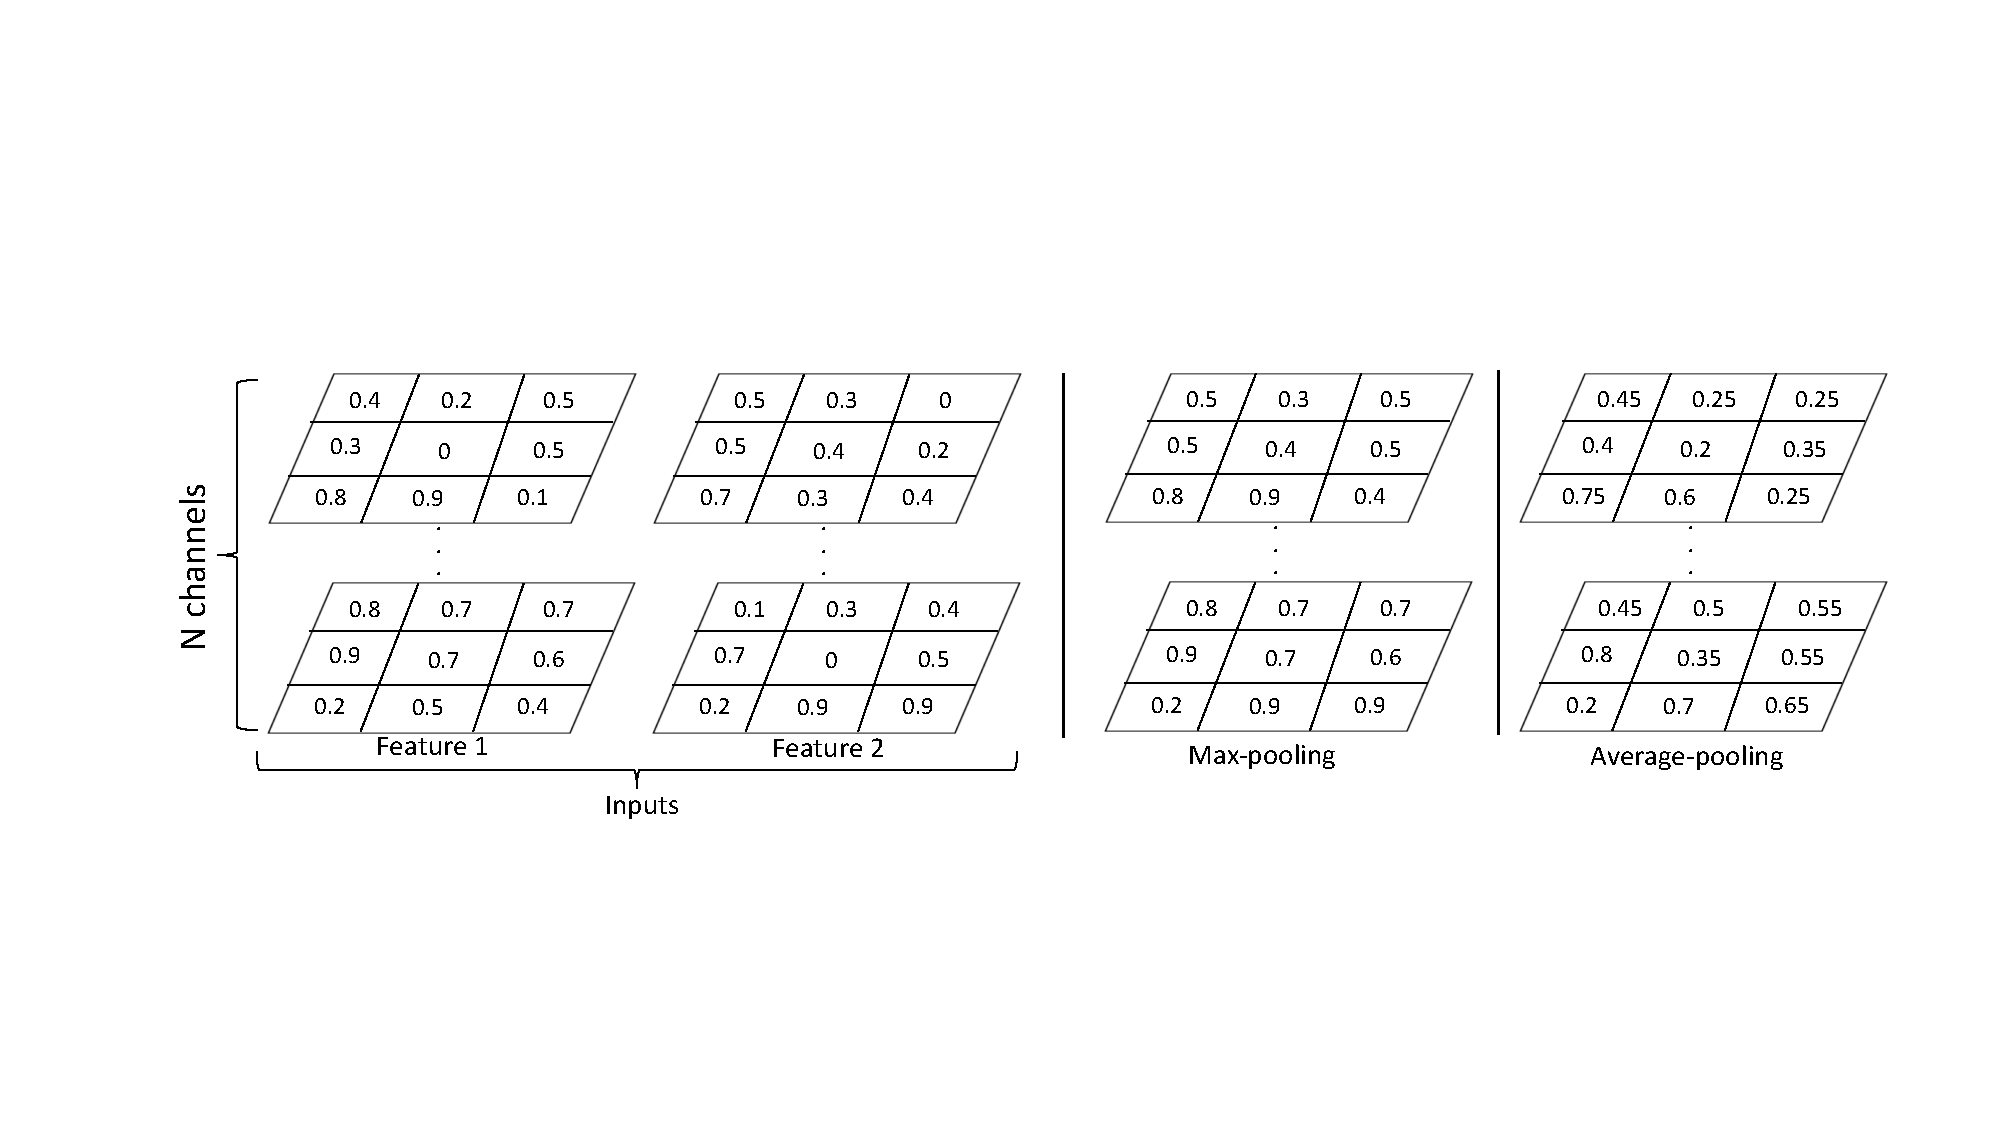
\includegraphics[width=\textwidth]{ch-psfcn/images/Method/pooling.pdf}
    \caption[Multi-feature fusion with max-pooling and average-pooling]{A toy example for max-pooling and average-pooling mechanisms on multi-feature fusion.} \label{fig:pooling}
\end{figure}

More recently, order-agnostic operations (\eg, pooling layers) have been exploited in CNNs to aggregate multi-image information. Wiles and Zisserman~\cite{wiles2017silnet} used max-pooling to fuse features of silhouettes from different views for novel view synthesis and 3D voxel prediction. Hartmann~\etal~\cite{hartmann2017learned} adopted average-pooling to aggregate features of multiple patches for learning multi-patch similarity. In general, max-pooling operation can extract the most salient information from all the features, while average-pooling can smooth out the salient and non-activated features. \fref{fig:pooling} illustrates how max-pooling and average-pooling operations aggregate two features with a toy example.  

For photometric stereo, we argue that max-pooling is a better choice for aggregating features from multiple inputs. 
Our motivation is that, under a certain light direction, regions with high intensities or specular highlights provide strong clues for surface normal inference (\eg, for a surface point with a sharp specular highlight, its normal is close to the bisector of the viewing and light directions). Max-pooling can naturally aggregate such strong features from images captured under different light directions. Besides, max-pooling can ignore non-activated features during training, making it robust to cast shadow. As will be seen in \Sref{sec:psfcn_exp}, our experimental results do validate our arguments. We observe from experiments that each channel of the feature map fused by max-pooling is highly correlated to the response of the surface to a certain light direction. Strong responses in each channel are found in regions with surface normals having similar directions. The feature map can therefore be interpreted as a decomposition of the images under different light directions (see \fref{fig:res_visual}).

\subsection{Network Architecture}
\label{sub:Network Architecture}

\begin{figure}[t] \centering
    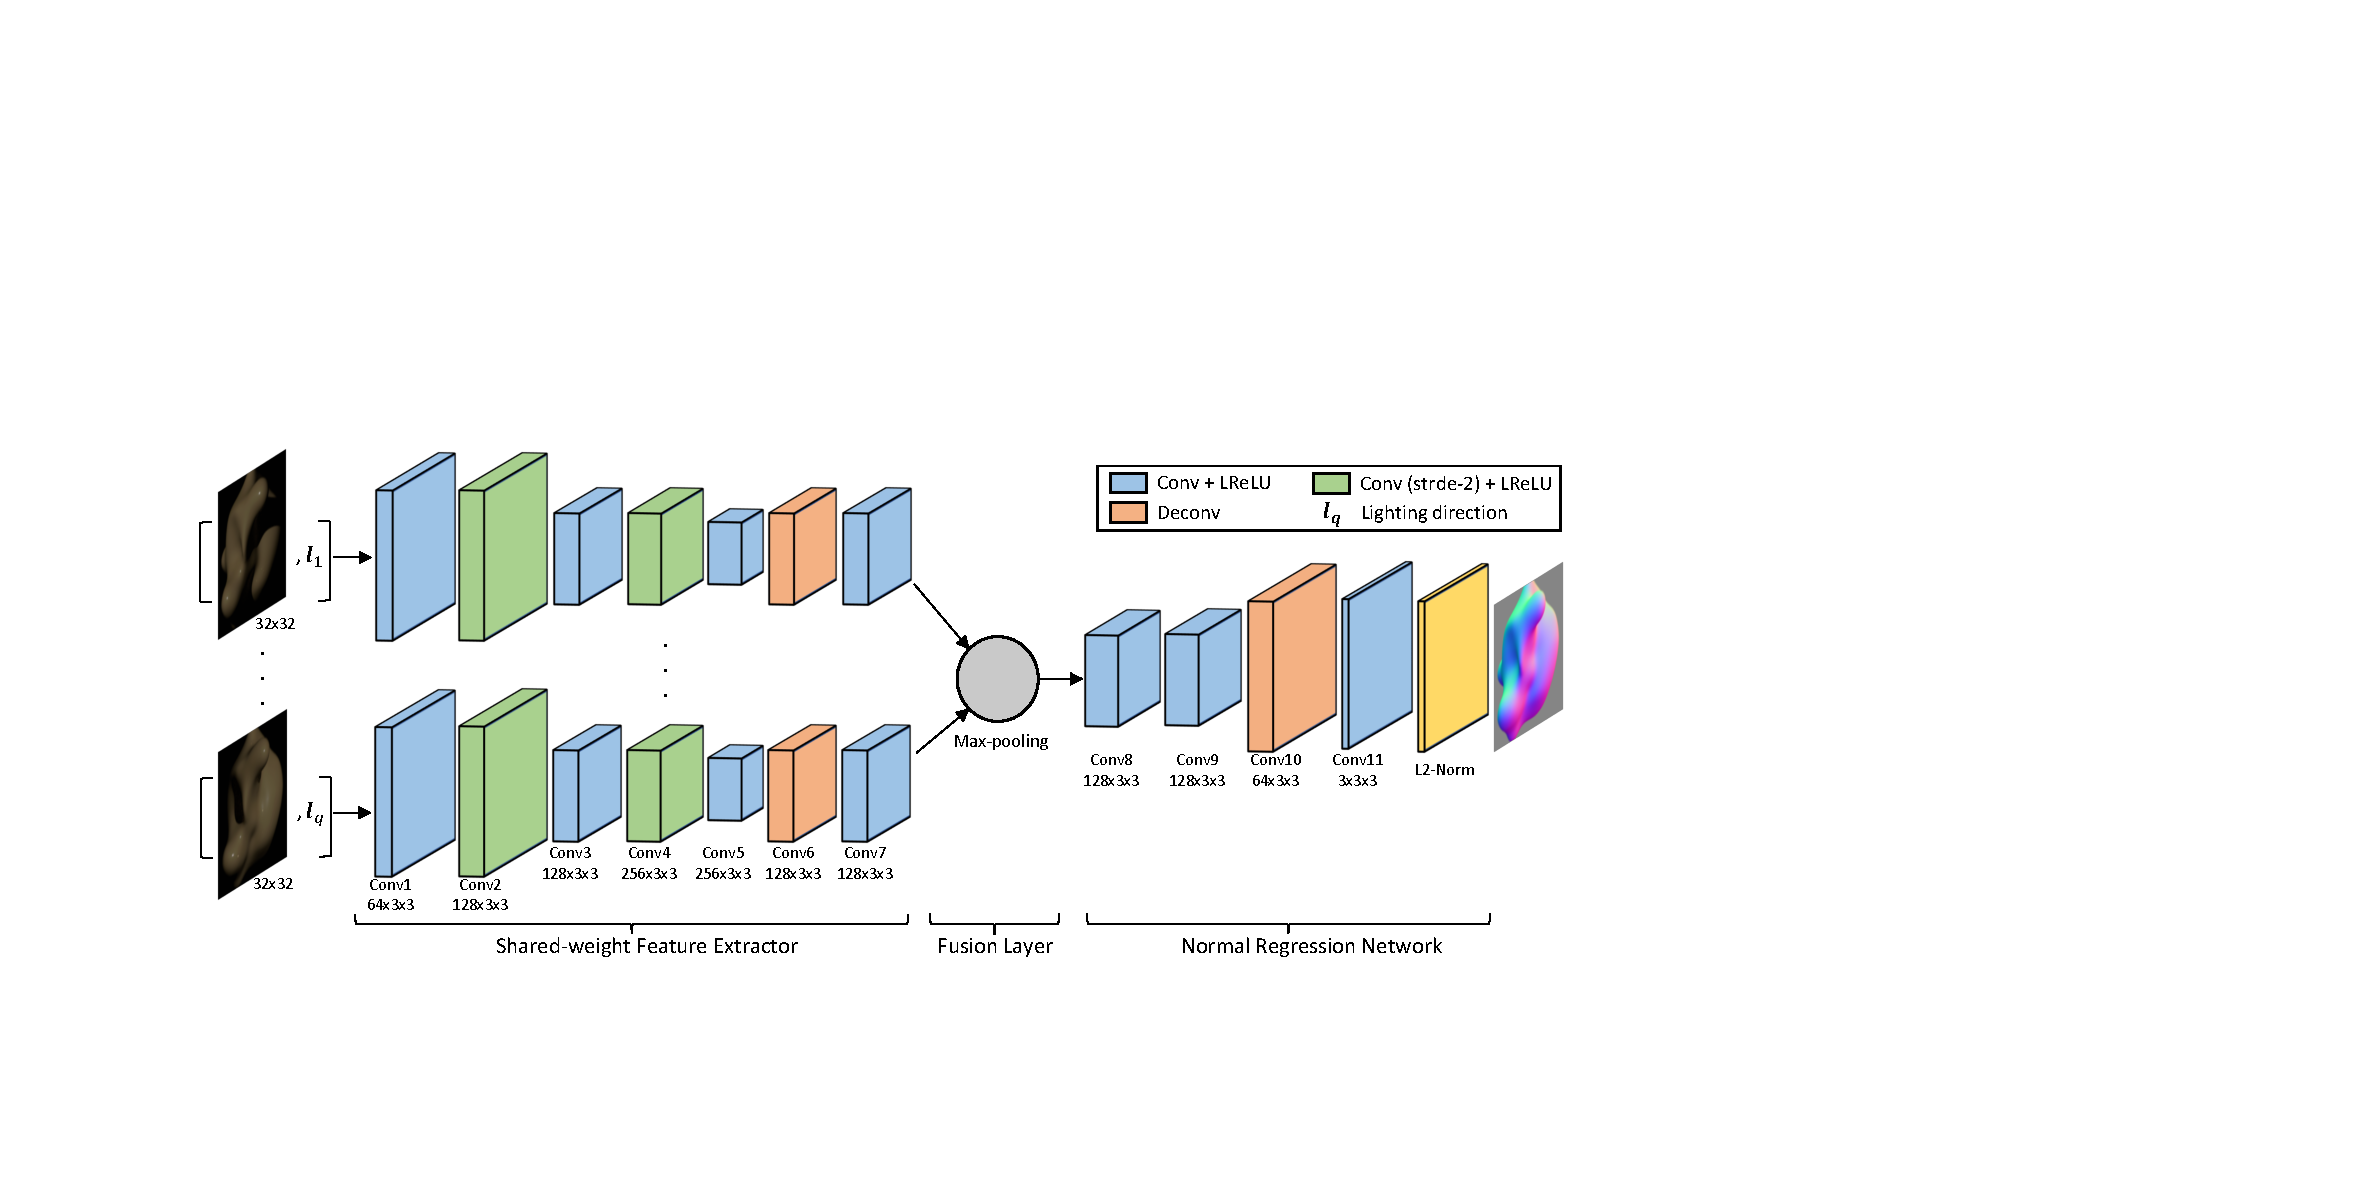
\includegraphics[width=\textwidth]{ch-psfcn/images/Method/network_v2}
    \caption{Network architecture of PS-FCN.} \label{fig:network}
\end{figure}

PS-FCN is a multi-input-single-output (MISO) network consisting of three components, namely a shared-weight \emph{feature extractor}, a \emph{fusion layer}, and a \emph{normal regression sub-network} (see \fref{fig:network}). It can be trained and tested using an arbitrary number of images with their associated light directions as input\footnote{For calibrated photometric stereo, the input images are normalized by light intensities, and each light direction is represented by a unit $3$-vector.}.

For each light direction, we have a $3$-channel input image with the dimensions of $3 \times h \times w$, where $h$ and $w$ are the image height and width, respectively. Concatenating images taken under $q$ different lightings $\{\vl_1, ..., \vl_q\}$, we have the data with the dimensions of $q \times 3 \times h \times w$. In addition, we represent the light vectors $\{\vl_1, ..., \vl_q\}$ as $3$-channel images having the same spatial resolution as the input images, resulting in another $q \times 3 \times h \times w$ data. Putting them together, we finally have $q \times 6 \times h \times w$ dimensional inputs to our model.
We separately feed the image-light pairs to the shared-weight feature extractor to extract a feature map from each of the inputs, and apply a max-pooling operation in the fusion layer to aggregate these feature maps. Finally, the normal regression sub-network takes the fused feature map as input and estimates a normal map of the object.

The shared-weight feature extractor has seven convolutional layers, where the feature map is down-sampled twice and then up-sampled once, resulting in a down-sample factor of two. This design can increase the receptive field and preserve spatial information with a small memory consumption. 
The normal regression sub-network has four convolutional layers and up-samples the fused feature map to the same spatial dimension as the input images. A L2-normalization layer is appended at the end of the normal regression sub-network to produce the normal map.

As PS-FCN is a fully convolutional network, it can be applied to datasets with different image sizes. Thanks to the max-pooling operation in the fusion layer, PS-FCN possesses an order-agnostic property. Besides, PS-FCN can be easily extended to handle uncalibrated photometric stereo, where the light directions are not known, by simply removing the light directions during training.

\paragraph{Loss function}
Training of our PS-FCN is supervised by the estimation error between the predicted and the ground-truth normal maps. We formulate our loss function as the commonly used cosine similarity loss, given by
\begin{align}
    \label{eq:normal}
    \mathcal{L}_{\text{Normal}} = \frac{1}{hw} \sum_{i}^{hw} \left(1 - \vn_i^\top \tilde{\vn}_{i} \right),
\end{align}
where $\vn_{i}$ and $\tilde{\vn}_{i}$ denote the predicted normal and the ground-truth normal, respectively, at pixel $i$.
If the predicted normal has a similar orientation as the ground truth, the dot-product $\vn_{i} \cdot \tilde{\vn}_{i}$ will be close to $1$ and the loss becomes small, and vice versa. Other losses like mean squared error can also be alternatively adopted.

\subsection{Data Normalization for Handling Surfaces with SVBRDFs}
As PS-FCN is a fully-convolutional network that processes the input images in a patch-wise manner and is trained on surfaces with homogeneous BRDF, it may have difficulties in dealing with steep color changes caused by surfaces with spatially-varying BRDFs (SVBRDFs), as shown in~\fref{fig:cat_SVBRDF}~(c).
A straightforward idea to tackle this problem is to train a model on surfaces with SVBRDFs. However, creating a large-scale training dataset for this purpose is not trivial, since modeling surface appearance with realistic SVBRDFs requires manual editing from artists.
Even someone can collect a large-scale dataset of objects with SVBRDFs, the created dataset may not be able to faithfully cover the distribution of real data. 
In this work, we introduce a simple yet effective data normalization strategy to enable PS-FCN to handle surfaces with SVBRDFs robustly. We will show that with the proposed data normalization strategy, our method can generalize well to surfaces with SVBRDFs after training only on surfaces with homogeneous BRDF.

\begin{figure}[tbp] \centering
        \makebox[0.190\textwidth]{\footnotesize (a) Object} 
    \makebox[0.190\textwidth]{\footnotesize (b) GT Normal} 
    \makebox[0.190\textwidth]{\footnotesize (c) PS-FCN} 
    \makebox[0.190\textwidth]{\footnotesize (d) PS-FCN$^{\text{+N}}$}
    \\
    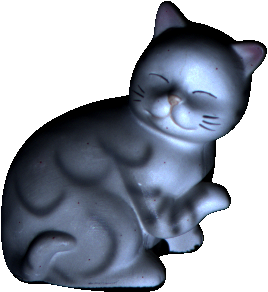
\includegraphics[width=0.190\textwidth]{ch-psfcn/images/Results/DiLiGenT/GT/4.0_catPNG_001.png}
    
\includegraphics[width=0.190\textwidth]{ch-psfcn/images/Results/DiLiGenT/GT/catPNGGT_normal.png}
    
\includegraphics[width=0.190\textwidth]{ch-psfcn/images/Results/DiLiGenT/PS-FCN/catPNGDiLiGenT_normal.png}
    
\includegraphics[width=0.190\textwidth]{ch-psfcn/images/Results/DiLiGenT/SVBRDF/PS-FCN_normalized/catPNGDiLiGenT_normal.png}
    \\
    \vspace{-1.2em}
    \makebox[0.190\textwidth]{} 
    \makebox[0.190\textwidth]{} 
    \makebox[0.190\textwidth]{\footnotesize \hfill (6.67)} 
    \makebox[0.190\textwidth]{\footnotesize \hfill (4.67)} 

    \caption[Comparison between PS-FCN and \PSFCNplusN on \emphobject{Cat} with SVBRDF]{Comparison between PS-FCN and \PSFCNplusN on \emphobject{Cat} with spatially-varying BRDFs. Numbers in parentheses denote mean angular error (MAE) in degree.} \label{fig:cat_SVBRDF}
\end{figure}

\begin{figure}[t] \centering
    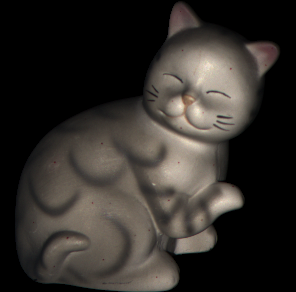
\includegraphics[width=0.150\textwidth]{ch-psfcn/images/Method/Cat_Normalized/4.0_004.png}
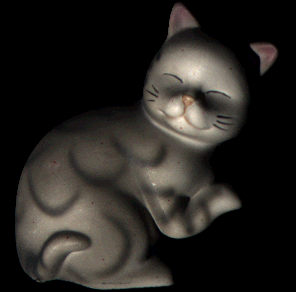
\includegraphics[width=0.150\textwidth]{ch-psfcn/images/Method/Cat_Normalized/4.0_041.png}
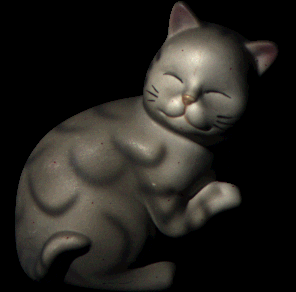
\includegraphics[width=0.150\textwidth]{ch-psfcn/images/Method/Cat_Normalized/4.0_048.png}
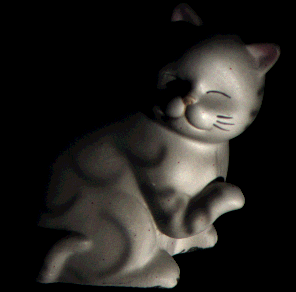
\includegraphics[width=0.150\textwidth]{ch-psfcn/images/Method/Cat_Normalized/4.0_089.png}
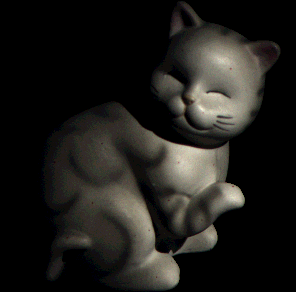
\includegraphics[width=0.150\textwidth]{ch-psfcn/images/Method/Cat_Normalized/4.0_096.png}
\\
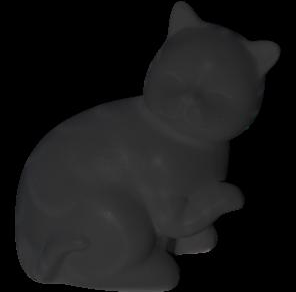
\includegraphics[width=0.150\textwidth]{ch-psfcn/images/Method/Cat_Normalized/4.0_1_2_3.png}
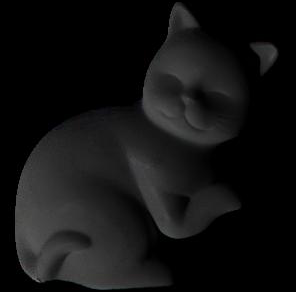
\includegraphics[width=0.150\textwidth]{ch-psfcn/images/Method/Cat_Normalized/4.0_1_2_40.png}
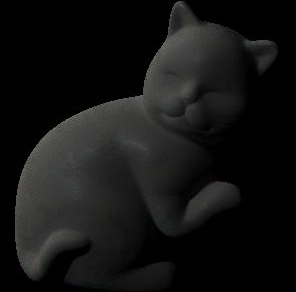
\includegraphics[width=0.150\textwidth]{ch-psfcn/images/Method/Cat_Normalized/4.0_1_2_47.png}
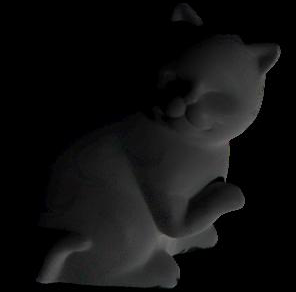
\includegraphics[width=0.150\textwidth]{ch-psfcn/images/Method/Cat_Normalized/4.0_1_2_88.png}
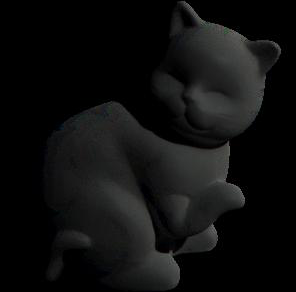
\includegraphics[width=0.150\textwidth]{ch-psfcn/images/Method/Cat_Normalized/4.0_1_2_95.png}
\\
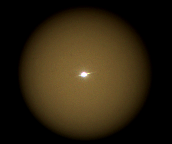
\includegraphics[width=0.150\textwidth]{ch-psfcn/images/Method/Ball_Normalized/4.0_004.png}
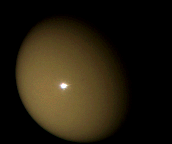
\includegraphics[width=0.150\textwidth]{ch-psfcn/images/Method/Ball_Normalized/4.0_041.png}
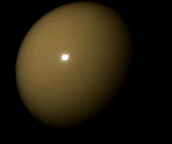
\includegraphics[width=0.150\textwidth]{ch-psfcn/images/Method/Ball_Normalized/4.0_048.png}
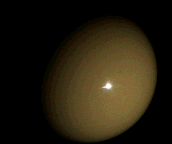
\includegraphics[width=0.150\textwidth]{ch-psfcn/images/Method/Ball_Normalized/4.0_089.png}
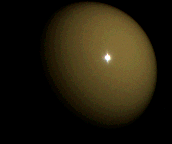
\includegraphics[width=0.150\textwidth]{ch-psfcn/images/Method/Ball_Normalized/4.0_096.png}
\\
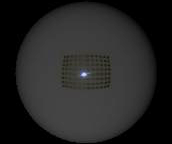
\includegraphics[width=0.150\textwidth]{ch-psfcn/images/Method/Ball_Normalized/4.0_1_1_3.png}
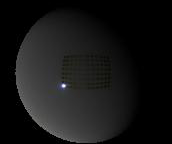
\includegraphics[width=0.150\textwidth]{ch-psfcn/images/Method/Ball_Normalized/4.0_1_1_40.png}
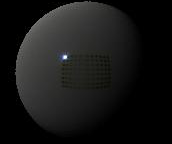
\includegraphics[width=0.150\textwidth]{ch-psfcn/images/Method/Ball_Normalized/4.0_1_1_47.png}
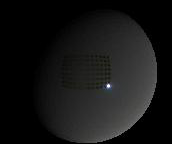
\includegraphics[width=0.150\textwidth]{ch-psfcn/images/Method/Ball_Normalized/4.0_1_1_88.png}
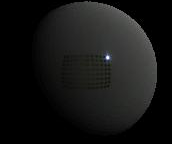
\includegraphics[width=0.150\textwidth]{ch-psfcn/images/Method/Ball_Normalized/4.0_1_1_95.png}
\\

    \caption[Illustration of the introduced data normalization operation]{Illustration of the introduced data normalization operation on \emphobject{cat} and \emphobject{ball} in the \diligent. The first and third rows show the original images, while the second and last rows show the normalized images. Only $5$ out of $96$ images for each object are shown.} \label{fig:normalization_SVBRDF}
\end{figure}

During training, given $q$ observations of a surface point\footnote{Note that the observations are already normalized by the light intensities.}, we concatenate all the observations and normalize them to a unit length vector by
\begin{align}
    \label{eq:normalize}
    \left(m_1', ..., m_{q}'\right) = \left(\frac{m_1}{\sqrt{m_1^2+...+m_{q}^2}}, ..., \frac{m_{q}}{\sqrt{m_1^2+...+m_{q}^2}}\right),
\end{align}
where $m$ and $m'$ represent the original and normalized observations, respectively (for RGB images, we perform normalization on each channel separately). 
The intuition behind this operation is as follows. Consider a Lambertian model, the BRDF $\rho(\vn, \vl)$ degenerates to a constant albedo $\rho$ and $m = \rho \max(\vn^\top \vl_j, 0)$. 
After the data normalization operation, we have
\begin{align}
    \label{eq:normalize2}
    m_{i}' = \frac{\max(\vn^\top \vl_i, 0)}{\sqrt{\max(\vn^\top \vl_1, 0)^2 + \cdots + \max(\vn^\top \vl_q, 0)^2}}.
\end{align}
\Eref{eq:normalize2} shows that the effect of albedo in Lambertian surfaces can be removed after performing data normalization, as shown in the first example in \fref{fig:normalization_SVBRDF}.

However, the above conclusion is not true for non-Lambertian surfaces, because for regions with specular highlights under some light directions, the observations under other light directions will be suppressed after data normalization (see the example of \emphobject{ball} in \fref{fig:normalization_SVBRDF}).
Nevertheless, we experimentally found that such a normalization strategy works equally well for non-Lambertian surfaces under the PS-FCN framework.
This might be explained by the fact that for a non-Lambertian surface under directional lighting, the low-frequency observations are quite close to Lambertian reflectance~\cite{shi2014bi}.
For observations exhibiting specular highlights under some light directions, the max-pooling operation in the fusion layer can naturally ignore the non-activated features (\ie, features extracted from the suppressed observations) and aggregate the most salient features.  
Note that this normalization strategy has also been adopted in~\cite{sato2007shape,lu2013uncalibrated} to compute the similarity between two pixel intensity profiles of non-Lambertian surfaces, while we use this normalization strategy as a preprocessing for CNNs to handle surfaces with SVBRDFs.  

When the number of input images at test time $t$ is different from that in training $q$, the magnitude of the normalized observations will be different, which leads to decreased performance (\eg, when all observations have the same values, 
we have $m_{\text{train}}' = 1/\sqrt{q}, m'_{\text{test}}=1/\sqrt{t}$). 
We experimentally verified that multiplying the normalized observations with the scalar $\sqrt{t/q}$ at test time solves this problem.
We trained a variant model of PS-FCN, denoted as \PSFCNplusN, using the proposed data normalization strategy.
\Fref{fig:cat_SVBRDF}~(d) shows an example result that \PSFCNplusN performed better than PS-FCN on surfaces with SVBRDFs.

\section{Dataset for Learning and Evaluation}
\label{sec:psfcn_dataset}
The training of PS-FCN requires the ground-truth normal maps of the objects. However, obtaining ground-truth normal maps of real objects is a difficult and time-consuming task. Hence, we create two synthetic datasets for training and one synthetic dataset for testing. The publicly available real photometric stereo datasets are reserved to validate the generalization ability of our model. Experimental results show that our PS-FCN trained on the synthetic datasets generalizes well on the challenging real datasets.

\subsection{Synthetic Data for Training}
We used shapes from two existing 3D datasets, namely the blobby shape dataset~\cite{johnson2011shape} and the sculpture shape dataset~\cite{wiles2017silnet}, to generate our training data using the physically based raytracer Mitsuba~\cite{jakob2010mitsuba}. Following DPSN~\cite{santo2017deep}, we employed the MERL dataset~\cite{matusik2003merl}, which contains 100 different BRDFs of real-world materials, to define a diverse set of surface materials for rendering these shapes. 
Note that our datasets explicitly consider cast shadows during rendering.
For the sake of data loading efficiency, we stored our training data in 8-bit PNG format.

\noindent{\bf Blobby dataset\enspace} We first followed~\cite{santo2017deep} to render our training data using the blobby shape dataset~\cite{johnson2011shape}, which contains 10 blobby shapes with various normal distributions. For each blobby shape, $1,296$ regularly-sampled views (36 azimuth angles $\times$ 36 elevation angles) were used, and for each view, 2 out of 100 BRDFs were randomly selected, leading to 25,920 samples ($10\times 36\times 36\times 2$).
For each sample, we rendered 64 images with a spatial resolution of $128 \times 128$ under light directions randomly sampled from a range of 180\degree $\times$ 180\degree, which is more general than the range (74.6\degree $\times$ 51.4\degree) used in the real data benchmark~\cite{shi2019benchmark}. We randomly split this dataset into $99:1$ for training and validation (see \fref{fig:data_samples}(a)).

\begin{figure} \centering
        \begin{subfigure}[t]{0.47\textwidth}
    \centering
    \makebox[0.225\textwidth]{\small (a) Blobby shape.}\\
    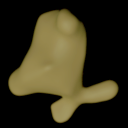
\includegraphics[width=0.235\textwidth]{ch-psfcn/images/Dataset/simple/l_000,-0.28,-0.27,0.92_gm.png}
    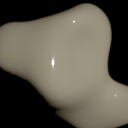
\includegraphics[width=0.235\textwidth]{ch-psfcn/images/Dataset/simple/l_002,0.60,0.12,0.79_gm.png}
    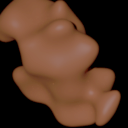
\includegraphics[width=0.235\textwidth]{ch-psfcn/images/Dataset/simple/l_006,-0.12,0.05,0.99_gm.png}
    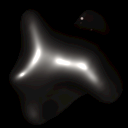
\includegraphics[width=0.235\textwidth]{ch-psfcn/images/Dataset/simple/l_022,-0.21,-0.20,0.96_gm.png}\\
    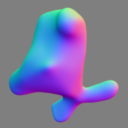
\includegraphics[width=0.235\textwidth]{ch-psfcn/images/Dataset/simple/blob06_s-0.80_x-250_y-250_normal.png}
    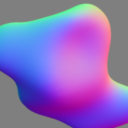
\includegraphics[width=0.235\textwidth]{ch-psfcn/images/Dataset/simple/blob02_s-1.00_x-250_y-250_normal.png}
    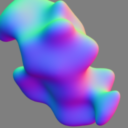
\includegraphics[width=0.235\textwidth]{ch-psfcn/images/Dataset/simple/blob08_s-0.80_x-250_y-250_normal.png}
    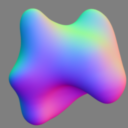
\includegraphics[width=0.235\textwidth]{ch-psfcn/images/Dataset/simple/blob07_s-0.90_x-250_y-250_normal.png}\\
    \end{subfigure}
    \quad
    \begin{subfigure}[t]{0.47\textwidth}
    \centering
    \makebox[0.225\textwidth]{\small (b) Sculpture shape.}\\
    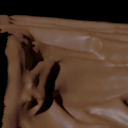
\includegraphics[width=0.235\textwidth]{ch-psfcn/images/Dataset/complex/l_000,-0.41,0.24,0.88_gm.png}
    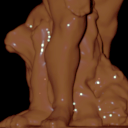
\includegraphics[width=0.235\textwidth]{ch-psfcn/images/Dataset/complex/l_001,-0.05,0.02,1.00_gm.png}
    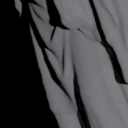
\includegraphics[width=0.235\textwidth]{ch-psfcn/images/Dataset/complex/l_005,0.25,0.03,0.97_gm.png}
    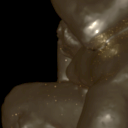
\includegraphics[width=0.235\textwidth]{ch-psfcn/images/Dataset/complex/l_012,-0.27,0.06,0.96_gm.png}
    \\
    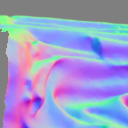
\includegraphics[width=0.235\textwidth]{ch-psfcn/images/Dataset/complex/virgin-mary-with-her-dead-son_alabasteryy_s-0.08_x-000_y-180_000_normal.png}
    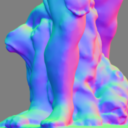
\includegraphics[width=0.235\textwidth]{ch-psfcn/images/Dataset/complex/wrestling-decimated-cleaned_aa-exported_s-0.06_x--90_y-100_010_normal.png}
    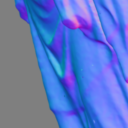
\includegraphics[width=0.235\textwidth]{ch-psfcn/images/Dataset/complex/virgin-and-child_model_s-0.25_x--90_y-100_006_normal.png}
    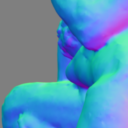
\includegraphics[width=0.235\textwidth]{ch-psfcn/images/Dataset/complex/ugolino-and-his-sons_zz_decimated_s-0.07_x-080_y-100_002_normal.png}\\
    \end{subfigure}

    \caption{Examples of the synthetic training data.}
    \label{fig:data_samples}
\end{figure}

\noindent{\bf Sculpture dataset\enspace} The surfaces in the blobby shape dataset are usually largely smooth and lack of details. To provide more complex (realistic) normal distributions for training, we employed 8 complicated 3D models from the sculpture shape dataset introduced in~\cite{wiles2017silnet}. We generated samples for the sculpture dataset in exactly the same way we did for the blobby shape dataset, except that  we discarded views containing holes or showing uniform normals (\eg, flat facets). 
The rendered images are with a size of $512 \times 512$ when a whole sculpture shape is in the field of view.
We then regularly cropped patches of size $128 \times 128$ from the rendered images and discarded those with a foreground ratio less than 50\%.\footnote{Each training image in the blobby dataset shows part of an object or a whole object depending on the viewpoint, whereas each training image in the sculpture dataset shows only part of an object since the sculpture shapes are much larger than the blobby shapes.}
This gave us a dataset of 59,292 samples, where each sample contains 64 images rendered under different light directions. Finally, we randomly split this dataset into $99:1$ for training and validation (see \fref{fig:data_samples}(b)).

\noindent{\bf Data augmentation\enspace} To narrow the gap between real and synthetic data, data augmentation was carried out on-the-fly during training. Given an image of size $128\times 128$, we randomly performed image rescaling (with the rescaled width and height within the range of $[32, 128]$, without preserving the original aspect ratio) and noise perturbation (in a range of $[-0.025, 0.025]$). Image patches of size $32\times 32$ were then randomly cropped for training. 

\begin{figure}[t] \centering
        \makebox[0.2\textwidth]{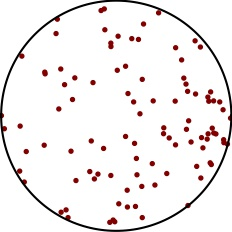
\includegraphics[width=0.110\textwidth]{ch-psfcn/images/Dataset/syn_test/MERL_directions}}
    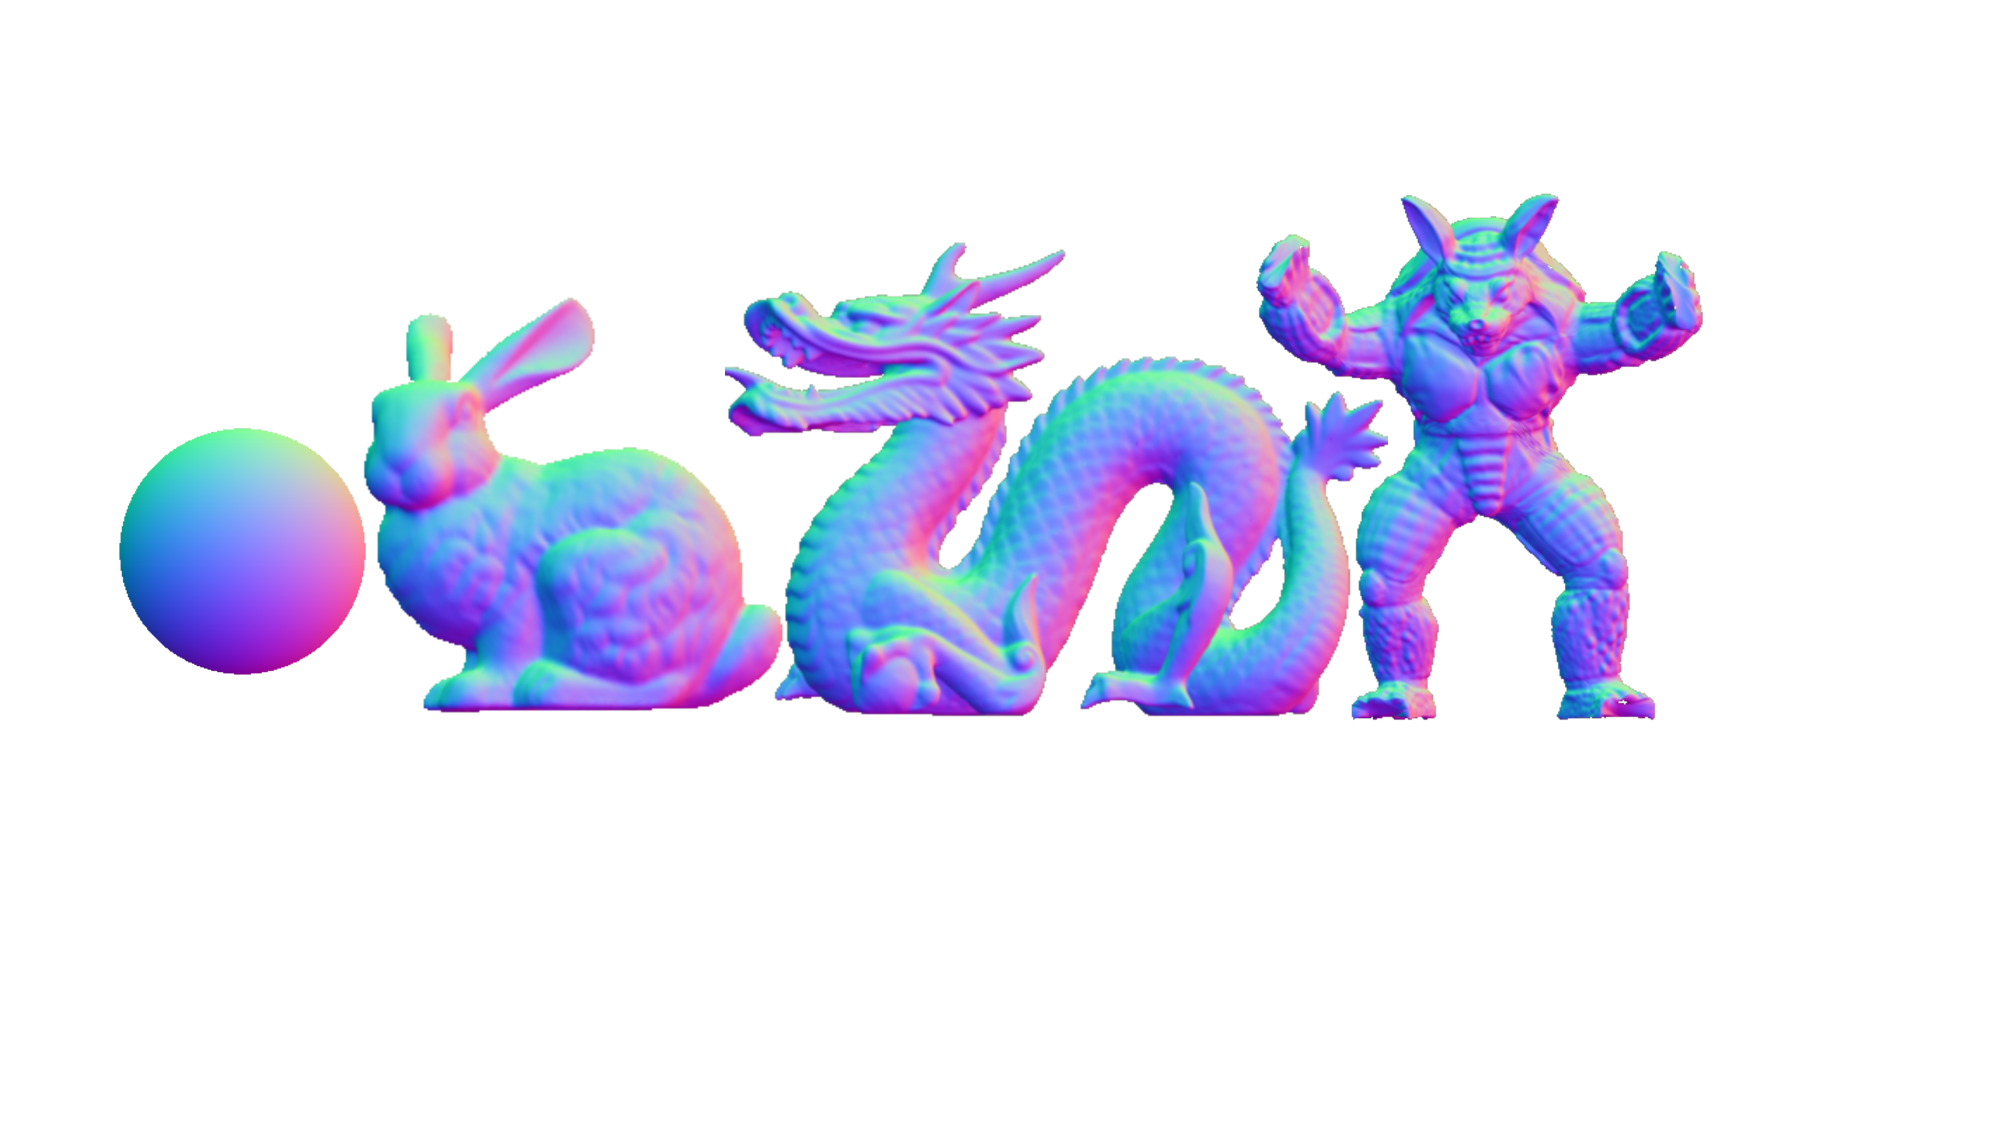
\includegraphics[width=0.60\textwidth]{ch-psfcn/images/Dataset/syn_test/synth_test_data.pdf}
    \\ \vspace{-0.3em}
    \makebox[0.20\textwidth]{\footnotesize (a) Light source} 
    \makebox[0.60\textwidth]{\footnotesize (b) {\sc Sphere}, {\sc Bunny}, {\sc Dragon} and {\sc Armadillo}} 
    \\
    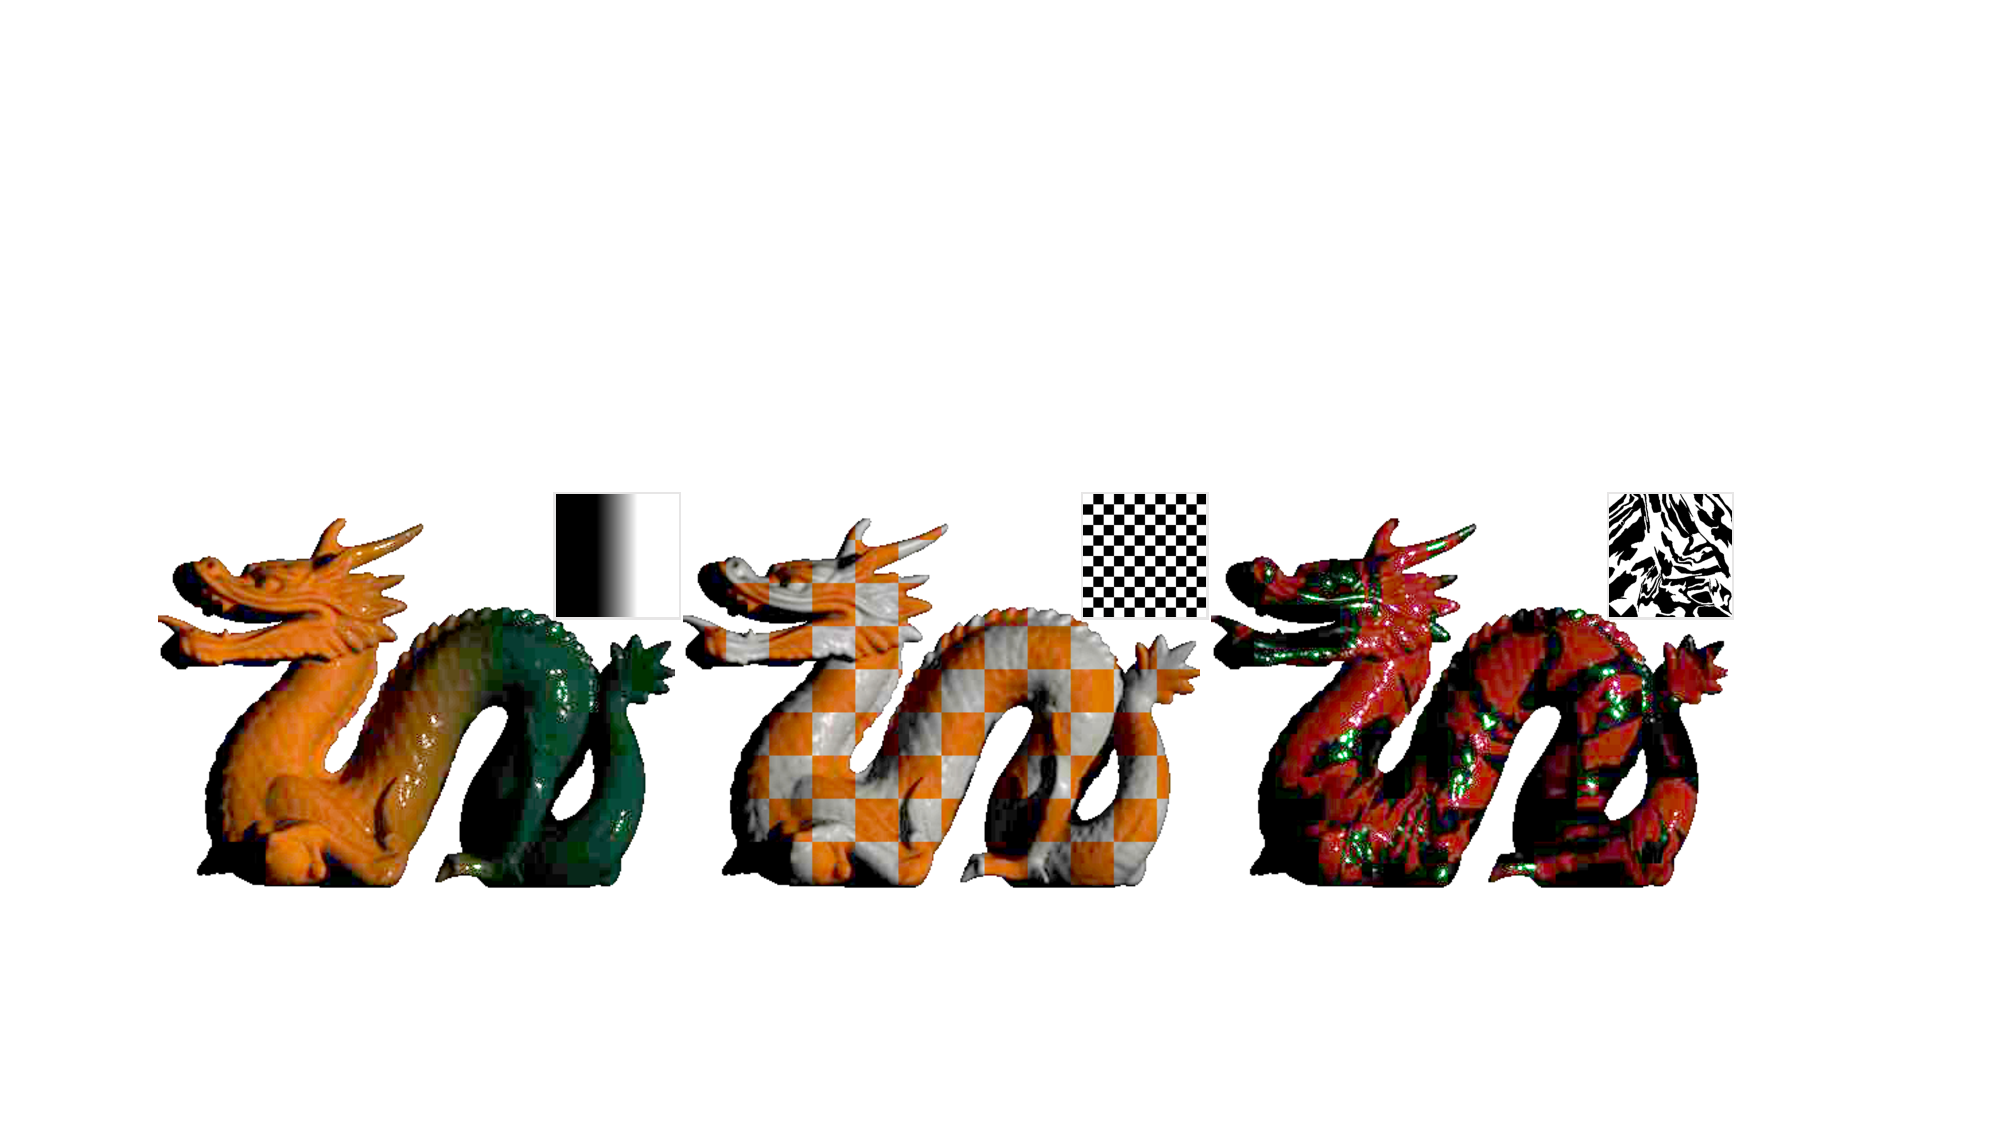
\includegraphics[width=0.7\textwidth]{ch-psfcn/images/Results/Synth_Test/SVBRDF/SVBRDF_Dragon.pdf} \\
    \makebox[0.48\textwidth]{\footnotesize (c) Example objects in {\sc Dragon$^\text{SVBRDF}$} dataset} \\

    \caption[Illustration of the synthetic test dataset \syntestMERL]{(a) Lighting distribution of \syntestMERL dataset. The light direction is visualized by mapping a $3$-d vector $[x,y,z]$ to a point $[x,y]$. (b) Ground-truth normals of \emphobject{Sphere}, \emphobject{Bunny}, \emphobject{Dragon}, and \emphobject{Armadillo}. (c) Visualization of the selected material maps (Ramp, Checker, Irregular) and examples in \dragonSVBRDF dataset.} \label{fig:syn_test_sample}
\end{figure}

\subsection{Synthetic Data for Analysis}
\label{subsec:synth_test_data}
To quantitatively evaluate the performance of our method on different materials and shapes, we rendered a synthetic test dataset including Sphere, Bunny, Dragon, and Armadillo shapes. Hereafter, we denote this test dataset as \syntestMERL and these shapes as \emphobject{Sphere}, \emphobject{Bunny}, \emphobject{Dragon}, \emphobject{Armadillo} respectively. 
Each shape was rendered with $100$ isotropic BRDFs from MERL dataset~\cite{matusik2003merl} under $100$ light directions randomly sampled from the upper-hemisphere, leading to $400$ test objects (see \fref{fig:syn_test_sample}~(a)-(b)).
Cast shadows and inter-reflections were considered during rendering using the physically based raytracer Mitsuba~\cite{jakob2010mitsuba}. 

To analyze how surfaces with SVBRDFs affect the performance of our method, we created another synthetic test dataset with SVBRDFs, denoted as \dragonSVBRDF, following~\cite{goldman2010shape}.
Specifically, we blended two BRDFs from $100$ MERL dataset for \emphobject{dragon} using $3$ materials maps, namely the \emph{Ramp}, \emph{Checker}, and \emph{Irregular}, as shown in \fref{fig:syn_test_sample}~(c). Note that for each material map, there are $C(100,2)=4,950$ combinations of two BRDFs, leading to $14,850$ test objects.

\begin{figure}[t] \centering
    \begin{minipage}{0.8\textwidth}
    \makebox[0.19\textwidth]{\footnotesize (a) DiLiGenT} 
    \makebox[0.19\textwidth]{\footnotesize (b) {\sc Apple}} 
    \makebox[0.19\textwidth]{\footnotesize (c) {\sc Gourd1}} 
    \makebox[0.19\textwidth]{\footnotesize (d) {\sc Gourd2}} 
    \makebox[0.19\textwidth]{\footnotesize (e) Light Stage} \\
    \makebox[0.19\textwidth]{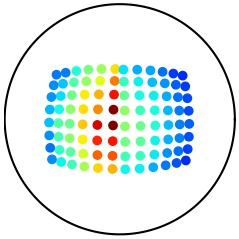
\includegraphics[width=0.15\textwidth]{ch-psfcn/images/Dataset/real/diligent_direction.jpg}}
    \makebox[0.19\textwidth]{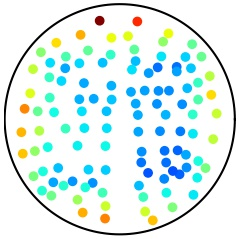
\includegraphics[width=0.15\textwidth]{ch-psfcn/images/Dataset/real/apple_direction.jpg}}
    \makebox[0.19\textwidth]{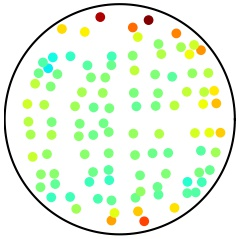
\includegraphics[width=0.15\textwidth]{ch-psfcn/images/Dataset/real/gourd1_direction.jpg}}
    \makebox[0.19\textwidth]{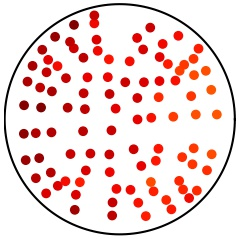
\includegraphics[width=0.15\textwidth]{ch-psfcn/images/Dataset/real/gourd2_direction.jpg}}
    \makebox[0.19\textwidth]{\includegraphics[width=0.15\textwidth]{ch-psfcn/images/Dataset/real/stage_direction.jpg}}
\end{minipage}
\begin{minipage}{0.02\textwidth}
     \centering
     \makebox[0.16\textwidth]{\scriptsize $0$}\\
     \vspace{0.1em}
     \includegraphics[width=0.55\linewidth]{ch-psfcn/images/Dataset/color_bar_jet} \\
     \vspace{-0.6em}
     \makebox[0.16\textwidth]{\scriptsize $1$}
\end{minipage}

    \caption[Lighting distributions of the real testing datasets]{Lighting distributions of the real testing datasets. The color of the point indicates the light intensity (value is divided by the highest intensity to normalize to $[0,1]$).} \label{fig:light_dist}
\end{figure}

\subsection{Real Data for Testing}
We employed three challenging real non-Lambertian photometric stereo datasets for testing, namely the \emph{\diligent}~\cite{shi2019benchmark}, \emph{\gourd}~\cite{alldrin2008p}, and \emph{\lightstage}~\cite{einarsson2006relighting}. Note that none of these datasets were used in the training.

\diligent~\cite{shi2019benchmark} is a public dataset containing $10$ real objects, and each object was captured under $96$ predefined light directions (see \fref{fig:light_dist}~(a)).  Both ground-truth lighting conditions and normal maps are provided. 
We quantitatively evaluated the performance of our method on both lighting and normal estimation.

Gourd\&Apple dataset~\cite{alldrin2008p} consists of three objects, namely \emphobject{Apple}, \emphobject{Gourd1}, and \emphobject{Gourd2}, with $112$, $102$ and $98$ images, respectively. 
\Frefs{fig:light_dist}~(b)-(d) visualize the lighting distributions of this dataset.  
\lightstage~\cite{einarsson2006relighting} is composed of six objects, and $253$ images are provided for each object. We only used $133$ images with the front side of the object under illumination. \Fref{fig:light_dist}~(e) visualizes the lighting distribution of the selected images.
Since these two datasets only provide calibrated lightings (without ground-truth normal maps), we quantitatively evaluated our method on lighting estimation but only qualitatively evaluated it on normal estimation.

\section{Experimental Results}
\label{sec:psfcn_exp}
In this section, we present experimental results and analysis. We carried out network analysis for PS-FCN on the synthetic test dataset, and compared our method with the previous state-of-the-art methods on the \diligent~\cite{shi2019benchmark}. Mean angular error (MAE) in degree was used to measure the accuracy of the predicted normal maps. We further provided qualitative results on the \gourd~\cite{alldrin2008p} and the \lightstage~\cite{einarsson2006relighting}. 

\paragraph{Implementation Details}
Our framework was implemented in PyTorch~\cite{paszke2017pytorch} with 2.2 million learnable parameters. 
We trained our model using a batch size of 32 for 30 epochs, and it only took a few hours for training to converge using a single NVIDIA Titan X Pascal GPU (\eg,  about 1 hour for 8 image-light pairs per sample on the blobby dataset, and about 9 hours for 32 image-light pairs per sample on both the blobby and sculpture datasets).
Adam optimizer~\cite{kingma2014adam} was used with default parameters ($\beta_1=0.9$ and $\beta_2=0.999$), where the learning rate was initially set to 0.001 and divided by 2 every 5 epochs. 

\subsection{Evaluation on Synthetic Data}
We quantitatively analyzed PS-FCN on the synthetic dataset. 
In particular, we first validated the effectiveness of max-pooling in multi-feature fusion by comparing it with average-pooling and convolutional layers.
We then investigated the influence of the complexity of training data, and the influence of input image number during training and testing. 
For all the experiments in network analysis, we performed $100$ random trials (save for the experiments using all $100$ image-light pairs per sample during testing) and reported the average results.
Last, we analyzed the performance of PS-FCN on surfaces with cast shadows, SVBRDFs, and different materials.

\begin{table}[htbp] \centering
    \caption[Normal estimation results of PS-FCN on \syntestMERL dataset]{Normal estimation results of different variant models of PS-FCN on \syntestMERL dataset. The results are averaged over samples rendered with $100$ BRDFs. B and S stand for the blobby and sculpture training datasets, respectively.} 
    \resizebox{0.8\textwidth}{!}{
    \Large
    \begin{tabular}{*{5}{c}|*{4}{c}}
        \toprule
        \multicolumn{5}{c}{Model Variants} & \multicolumn{4}{c}{Test Objects} \\
        ID & Data & Fusion &  Train \# & Test \# & {\sc Sphere} & {\sc Bunny} & {\sc Dragon} & {\sc Armod.} \\
        \midrule
        A0 & B   & Conv  & 32 & 32  & 4.54 & 6.74 & 9.57 & 9.87 \\
        A1 & B   & Max-p & 32 & 32  & 3.65 & 5.33 & 7.86 & 8.09 \\
        \midrule               
        A2 & B   & Avg-p & 32 & 100 & 3.71 & 5.36 & 8.17 & 7.92 \\
        A3 & B   & Max-p & 32 & 100 & 3.40 & 4.80 & 7.23 & 7.21 \\
        \midrule               
        A4 & B+S & Max-p & 32 & 100 & \B{2.66} & \B{3.80} & \B{4.83} & \B{5.24} \\
        \bottomrule
    \end{tabular}
}
 \label{tab:quant_calib_normal_syn}
\end{table}

\paragraph{Effectiveness of max-pooling} We first validated the effectiveness of max-pooling in multi-feature fusion by comparing it with convolutional layers and average-pooling. 
Experiments with IDs A0 \& A1 in \Tref{tab:quant_calib_normal_syn} show that fusion by convolutional layer on the concatenated features was sub-optimal. This could be explained by the fact that the weights of the convolutional layer are related to the order of the input features, while the order of the input image-light pairs is random in our case, thus increasing the difficulty for the convolutional layer to find the relations among multiple features. 
Experiments with IDs A2 \& A3 compared the performance of average-pooling and max-pooling for multi-feature fusion. It can be seen that max-pooling performs consistently better than average-pooling on \syntestMERL dataset.
\Fref{fig:res_visual} visualizes the fused features by max-pooling for four objects with different shapes and reflectances. We can see that each channel of the fused features can be interpreted as the probability of the normal belonging to a certain direction, and max-pooling can naturally aggregate such information from multiple observations.

\begin{figure}[htbp]
\centering
    \begin{minipage}{0.97\textwidth}
    \makebox[0.092\textwidth]{\footnotesize Obj} 
    \makebox[0.092\textwidth]{\footnotesize GT} 
    \makebox[0.092\textwidth]{\footnotesize (a)} 
    \makebox[0.092\textwidth]{\footnotesize (b)}
    \makebox[0.092\textwidth]{\footnotesize (c)} 
    \makebox[0.092\textwidth]{\footnotesize (d)} 
    \makebox[0.092\textwidth]{\footnotesize (e)} 
    \makebox[0.092\textwidth]{\footnotesize (f)} 
    \makebox[0.092\textwidth]{\footnotesize (g)} 
    \makebox[0.092\textwidth]{\footnotesize (h)} 
 \\
 \includegraphics[width=0.092\textwidth]{ch-psfcn/images/Results/visual_new/sphere_blue_rubber.png}
 \includegraphics[width=0.092\textwidth]{ch-psfcn/images/Results/visual_new/sphere_normal.png}
 \includegraphics[width=0.092\textwidth]{ch-psfcn/images/Results/visual_new/sphere_s-0.80_x-000_y-000_blue-rubber_40.jpg}
 \includegraphics[width=0.092\textwidth]{ch-psfcn/images/Results/visual_new/sphere_s-0.80_x-000_y-000_blue-rubber_31.jpg}
 \includegraphics[width=0.092\textwidth]{ch-psfcn/images/Results/visual_new/sphere_s-0.80_x-000_y-000_blue-rubber_25.jpg}
 \includegraphics[width=0.092\textwidth]{ch-psfcn/images/Results/visual_new/sphere_s-0.80_x-000_y-000_blue-rubber_5.jpg}
 \includegraphics[width=0.092\textwidth]{ch-psfcn/images/Results/visual_new/sphere_s-0.80_x-000_y-000_blue-rubber_0.jpg}
 \includegraphics[width=0.092\textwidth]{ch-psfcn/images/Results/visual_new/sphere_s-0.80_x-000_y-000_blue-rubber_35.jpg}
 \includegraphics[width=0.092\textwidth]{ch-psfcn/images/Results/visual_new/sphere_s-0.80_x-000_y-000_blue-rubber_41.jpg}
 \includegraphics[width=0.092\textwidth]{ch-psfcn/images/Results/visual_new/sphere_s-0.80_x-000_y-000_blue-rubber_24.jpg}
 \\
 \includegraphics[width=0.092\textwidth]{ch-psfcn/images/Results/visual_new/bunny_dark-red-paint.png}
 \includegraphics[width=0.092\textwidth]{ch-psfcn/images/Results/visual_new/bunny_normal.png}
 \includegraphics[width=0.092\textwidth]{ch-psfcn/images/Results/visual_new/bunny_s-0.55_x-000_y-180_green-latex_40.jpg}
 \includegraphics[width=0.092\textwidth]{ch-psfcn/images/Results/visual_new/bunny_s-0.55_x-000_y-180_green-latex_31.jpg}
 \includegraphics[width=0.092\textwidth]{ch-psfcn/images/Results/visual_new/bunny_s-0.55_x-000_y-180_green-latex_25.jpg}
 \includegraphics[width=0.092\textwidth]{ch-psfcn/images/Results/visual_new/bunny_s-0.55_x-000_y-180_green-latex_5.jpg}
 \includegraphics[width=0.092\textwidth]{ch-psfcn/images/Results/visual_new/bunny_s-0.55_x-000_y-180_green-latex_0.jpg}
 \includegraphics[width=0.092\textwidth]{ch-psfcn/images/Results/visual_new/bunny_s-0.55_x-000_y-180_green-latex_35.jpg}
 \includegraphics[width=0.092\textwidth]{ch-psfcn/images/Results/visual_new/bunny_s-0.55_x-000_y-180_green-latex_41.jpg}
 \includegraphics[width=0.092\textwidth]{ch-psfcn/images/Results/visual_new/bunny_s-0.55_x-000_y-180_green-latex_24.jpg}
 \\
 \includegraphics[width=0.092\textwidth]{ch-psfcn/images/Results/DiLiGenT/main_qual_img/4.0_pot2PNG_001.png}
 \includegraphics[width=0.092\textwidth]{ch-psfcn/images/Results/DiLiGenT/GT/1_5_1.jpg}
 \includegraphics[width=0.092\textwidth]{ch-psfcn/images/Results/visual_new/pot2PNG_40.jpg}
 \includegraphics[width=0.092\textwidth]{ch-psfcn/images/Results/visual_new/pot2PNG_31.jpg}
 \includegraphics[width=0.092\textwidth]{ch-psfcn/images/Results/visual_new/pot2PNG_25.jpg}
 \includegraphics[width=0.092\textwidth]{ch-psfcn/images/Results/visual_new/pot2PNG_5.jpg}
 \includegraphics[width=0.092\textwidth]{ch-psfcn/images/Results/visual_new/pot2PNG_0.jpg}
 \includegraphics[width=0.092\textwidth]{ch-psfcn/images/Results/visual_new/pot2PNG_35.jpg}
 \includegraphics[width=0.092\textwidth]{ch-psfcn/images/Results/visual_new/pot2PNG_41.jpg}
 \includegraphics[width=0.092\textwidth]{ch-psfcn/images/Results/visual_new/pot2PNG_24.jpg}
 \\
 \includegraphics[width=0.092\textwidth]{ch-psfcn/images/Results/DiLiGenT/main_qual_img/3.0_bearPNG_001.png}
 \includegraphics[width=0.092\textwidth]{ch-psfcn/images/Results/DiLiGenT/GT/1_4_1.jpg}
 \includegraphics[width=0.092\textwidth]{ch-psfcn/images/Results/visual_new/bearPNG_40.jpg}
 \includegraphics[width=0.092\textwidth]{ch-psfcn/images/Results/visual_new/bearPNG_31.jpg}
 \includegraphics[width=0.092\textwidth]{ch-psfcn/images/Results/visual_new/bearPNG_25.jpg}
 \includegraphics[width=0.092\textwidth]{ch-psfcn/images/Results/visual_new/bearPNG_5.jpg}
 \includegraphics[width=0.092\textwidth]{ch-psfcn/images/Results/visual_new/bearPNG_0.jpg}
 \includegraphics[width=0.092\textwidth]{ch-psfcn/images/Results/visual_new/bearPNG_35.jpg}
 \includegraphics[width=0.092\textwidth]{ch-psfcn/images/Results/visual_new/bearPNG_41.jpg}
 \includegraphics[width=0.092\textwidth]{ch-psfcn/images/Results/visual_new/bearPNG_24.jpg}
\end{minipage} %
\begin{minipage}{0.012\textwidth}
     \centering
     \makebox[0.16\textwidth]{\scriptsize  $0$}\\
     \vspace{0.2em}
     \includegraphics[width=\textwidth]{ch-psfcn/images/Results/visual_new/color_bar} \\
     \vspace{-0.4em}
     \makebox[0.16\textwidth]{\scriptsize $1$}
\end{minipage}

    \caption[Visualization of the learned feature map after fusion]{Visualization of the learned feature map after fusion. The first two columns show the images and ground-truth normal maps. Each of the subsequent columns (a-h) shows one particular channel of the fused feature map. 8 out of the 128 channels of the feature map are presented. Note that different regions with similar normal directions are fired in different channels. Each channel can therefore be interpreted as the probability of the normal belonging to a certain direction (or alternatively as the object shading rendered under a certain light direction). Accurate normal maps can then be inferred from these probability distributions.} \label{fig:res_visual}
\end{figure}

\begin{figure}[htbp] \centering
    \includegraphics[width=0.45\textwidth]{ch-psfcn/images/Results/Synth_Test/train_normal_img_num_sensitivity_v3.pdf}
    \includegraphics[width=0.45\textwidth]{ch-psfcn/images/Results/Synth_Test/test_normal_img_num_sensitivity.pdf} 
    \\ \vspace{-0.5em}
    \makebox[0.45\textwidth]{\footnotesize (a)} 
    \makebox[0.45\textwidth]{\footnotesize (b)} \\
    \caption[Effect of the input image number]{(a) Results of PS-FCN trained and tested with different numbers of input images on \emphobject{Sphere}. (b) Results of PS-FCN trained with a fixed number of $32$ input images and tested with different numbers of input images.} 
    \label{fig:calib_img_num_syn}
\end{figure}

\paragraph{Effects of training data and input image number} 
By comparing experiments with ID A3 \& A4 in \Tref{tab:quant_calib_normal_syn}, we can see that training with the additional sculpture dataset that has a more complex normal distribution helped to boost the performance of PS-FCN. This result suggests that the performance of PS-FCN could be further improved by introducing more complex and realistic training data. 

\Fref{fig:calib_img_num_syn}~(a) shows that for a fixed number of inputs during testing, PS-FCN performs better when the number of inputs during training is close to that during testing. 
It is worth noting that when there is only one input image, the problem reduces to the more challenging shape-from-shading problem. \Fref{fig:calib_img_num_syn}~(a) shows that PS-FCN performs best when the training image number is also $1$, with an average MAE of $18.75\degree$ for \emphobject{Sphere}. However, this result is moderately inaccurate, indicating that PS-FCN has difficulties in resolving the ambiguity in the problem of shape from shading.

\Fref{fig:calib_img_num_syn}~(b) shows that for a fixed number of inputs during training, the performance of PS-FCN increases with the number of inputs during testing. This is a desired property for photometric stereo as we can simply capture more images for robust estimation. 
For the rest of this chapter, we refer PS-FCN as the model trained on both datasets and with an input of $32$ image-light pairs per sample.

\paragraph{Effects of lighting distributions} We tested PS-FCN on \emphobject{Bunny} rendered with three different lighting distributions, as shown in \Tref{tab:res_synth_mirco_baseline}. These three distributions have the same number of light source (\ie, $17$), but with different spanning ranges.
We can see that PS-FCN performs better when lightings are more diversely distributed. For the highly clustered distribution (see \Tref{tab:res_synth_mirco_baseline}~(c)), the results of PS-FCN drops notably. Since the lightings are randomly sampled from the upper-hemisphere (\ie, spanning range of $180\degree \times 180\degree$) during training, it is therefore not surprising to see PS-FCN with decreased performance under this extreme lighting distribution.

\begin{table}[htbp] \centering
    \caption[Results on \emphobject{Bunny} rendered using three different lighting distributions]{Results of PS-FCN on \emphobject{Bunny} rendered using three different lighting distributions.} 
    \label{tab:res_synth_mirco_baseline}
    \includegraphics[width=0.15\textwidth]{ch-psfcn/images/Results/Micro_Baseline/uniform_17.jpg}
\includegraphics[width=0.15\textwidth]{ch-psfcn/images/Results/Micro_Baseline/uniform_17_3.00.jpg}
\includegraphics[width=0.15\textwidth]{ch-psfcn/images/Results/Micro_Baseline/uniform_17_8.00.jpg}
\raisebox{0.9\height}{
\resizebox{0.3\textwidth}{!}{
\large
\begin{tabular}{ccc}
    \toprule
    Type & Range & MAE \\
    \midrule
    (a) & 144\degree$\times$144\degree & 4.21 \\ 
    (b) & 37\degree$\times$37\degree & 10.90 \\
    (c) & 22\degree$\times$22\degree & 18.72 \\
    \bottomrule
\end{tabular}
}}
\\
\vspace{-0.2em}
\makebox[0.15\textwidth]{\footnotesize (a)} 
\makebox[0.15\textwidth]{\footnotesize (b)}
\makebox[0.15\textwidth]{\footnotesize (c)}
\makebox[0.30\textwidth]{\footnotesize (d) Normal estimation}
\\

\end{table}

\paragraph{Results on surface with cast shadows} 
\begin{figure}[htbp] \centering
    \begin{subfigure}[t]{0.9\textwidth}
         \makebox[0.16\textwidth]{\footnotesize Image 1} 
 \makebox[0.16\textwidth]{\footnotesize Image 2} 
 \makebox[0.16\textwidth]{\footnotesize Image 3} 
 \makebox[0.16\textwidth]{\footnotesize Image 4} 
 \makebox[0.16\textwidth]{\footnotesize Image 5} 
 \hfill
 \makebox[0.16\textwidth]{\footnotesize Fused Feat.} 
 \\
 \includegraphics[width=0.16\textwidth]{ch-psfcn/images/Results/Cast_Shadow/2.5_feat_048_v2.png}
 \includegraphics[width=0.16\textwidth]{ch-psfcn/images/Results/Cast_Shadow/2.5_feat_008_v2.png}
 \includegraphics[width=0.16\textwidth]{ch-psfcn/images/Results/Cast_Shadow/2.5_feat_021_v2.png}
 \includegraphics[width=0.16\textwidth]{ch-psfcn/images/Results/Cast_Shadow/2.5_feat_096_v2.png}
 \includegraphics[width=0.16\textwidth]{ch-psfcn/images/Results/Cast_Shadow/2.5_feat_089_v2.png}
 \hfill
 \includegraphics[width=0.16\textwidth]{ch-psfcn/images/Results/Cast_Shadow/mask.png}
 \\
 \includegraphics[width=0.16\textwidth]{ch-psfcn/images/Results/Cast_Shadow/gobletPNG_0_3.jpg}
 \includegraphics[width=0.16\textwidth]{ch-psfcn/images/Results/Cast_Shadow/gobletPNG_3_3.jpg}
 \includegraphics[width=0.16\textwidth]{ch-psfcn/images/Results/Cast_Shadow/gobletPNG_4_3.jpg}
 \includegraphics[width=0.16\textwidth]{ch-psfcn/images/Results/Cast_Shadow/gobletPNG_7_3.jpg}
 \includegraphics[width=0.16\textwidth]{ch-psfcn/images/Results/Cast_Shadow/gobletPNG_9_3.jpg}
 \hfill
 \includegraphics[width=0.16\textwidth]{ch-psfcn/images/Results/Cast_Shadow/gobletPNG_3.jpg}
 \\
 \includegraphics[width=0.16\textwidth]{ch-psfcn/images/Results/Cast_Shadow/gobletPNG_0_21.jpg}
 \includegraphics[width=0.16\textwidth]{ch-psfcn/images/Results/Cast_Shadow/gobletPNG_3_21.jpg}
 \includegraphics[width=0.16\textwidth]{ch-psfcn/images/Results/Cast_Shadow/gobletPNG_4_21.jpg}
 \includegraphics[width=0.16\textwidth]{ch-psfcn/images/Results/Cast_Shadow/gobletPNG_7_21.jpg}
 \includegraphics[width=0.16\textwidth]{ch-psfcn/images/Results/Cast_Shadow/gobletPNG_9_21.jpg}
 \hfill
 \includegraphics[width=0.16\textwidth]{ch-psfcn/images/Results/Cast_Shadow/gobletPNG_21.jpg} 
 \\
 \includegraphics[width=0.16\textwidth]{ch-psfcn/images/Results/Cast_Shadow/gobletPNG_0_103.jpg}
 \includegraphics[width=0.16\textwidth]{ch-psfcn/images/Results/Cast_Shadow/gobletPNG_3_103.jpg}
 \includegraphics[width=0.16\textwidth]{ch-psfcn/images/Results/Cast_Shadow/gobletPNG_4_103.jpg}
 \includegraphics[width=0.16\textwidth]{ch-psfcn/images/Results/Cast_Shadow/gobletPNG_7_103.jpg}
 \includegraphics[width=0.16\textwidth]{ch-psfcn/images/Results/Cast_Shadow/gobletPNG_9_103.jpg}
 \hfill
 \includegraphics[width=0.16\textwidth]{ch-psfcn/images/Results/Cast_Shadow/gobletPNG_103.jpg} 
 \\
\vspace{-1.5em}
        \caption{The first five columns show the input images and the extracted features for each image (only $3$ out of $128$ feature channels are shown). The last column shows the object mask and the fused features by max-pooling. Red boxes in the images indicate regions with cast shadows.} \label{fig:visual_cast_shadow}
    \end{subfigure} \\ \vspace{1em}
    \begin{subfigure}[t]{0.8\textwidth}
        \begin{minipage}{0.97\textwidth}
 \makebox[0.243\textwidth]{\footnotesize GT / Object} 
 \makebox[0.243\textwidth]{\footnotesize PS-FCN} 
 \makebox[0.243\textwidth]{\footnotesize SS17~\cite{santo2017deep}} 
 \makebox[0.243\textwidth]{\footnotesize L2 Baseline~\cite{woodham1980ps}} 
 \\
 \includegraphics[width=0.243\textwidth]{ch-psfcn/images/Results/DiLiGenT/GT/gobletPNGGT_normal_box.png}
 \includegraphics[width=0.243\textwidth]{ch-psfcn/images/Results/DiLiGenT/PS-FCN/gobletPNGDiLiGenT_normal.png}
 \includegraphics[width=0.243\textwidth]{ch-psfcn/images/Results/DiLiGenT/DPSN/goblet_normal.png}
 \includegraphics[width=0.243\textwidth]{ch-psfcn/images/Results/DiLiGenT/L2/gobletPNGl2_normal.png}
 \\
 \includegraphics[width=0.243\textwidth]{ch-psfcn/images/Results/DiLiGenT/GT/4.0_gobletPNG_001.png}
 \includegraphics[width=0.243\textwidth]{ch-psfcn/images/Results/DiLiGenT/PS-FCN/gobletPNGDiLiGenT_diff.png}
 \includegraphics[width=0.243\textwidth]{ch-psfcn/images/Results/DiLiGenT/DPSN/goblet_diff.png}
 \includegraphics[width=0.243\textwidth]{ch-psfcn/images/Results/DiLiGenT/L2/gobletPNGl2_diff.png}
 \vspace{-2.7em}
 \\
 \makebox[0.243\textwidth]{\footnotesize } 
 \makebox[0.243\textwidth]{\footnotesize \hfill (8.6)} 
 \makebox[0.243\textwidth]{\footnotesize \hfill (11.3)} 
 \makebox[0.243\textwidth]{\footnotesize \hfill (18.5)} 
 \vspace{-0.8em}
 \\
 \includegraphics[width=0.110\textwidth]{ch-psfcn/images/Results/goblet_crop/gobletPNGGT_normal_crop.png}\hspace{-0.2em}
    \includegraphics[width=0.110\textwidth]{ch-psfcn/images/Results/goblet_crop/4.0_gobletPNG_001_crop.png}
    \hfill
    \includegraphics[width=0.110\textwidth]{ch-psfcn/images/Results/goblet_crop/gobletPNGDiLiGenT_normal_crop.png}\hspace{-0.2em}
    \includegraphics[width=0.110\textwidth]{ch-psfcn/images/Results/goblet_crop/gobletPNGDiLiGenT_diff_crop.png}
    \hfill
    \includegraphics[width=0.110\textwidth]{ch-psfcn/images/Results/goblet_crop/goblet_normal_DPSN_crop.png}\hspace{-0.2em}
    \includegraphics[width=0.110\textwidth]{ch-psfcn/images/Results/goblet_crop/goblet_diff_DPSN_crop.png}
    \hfill
    \includegraphics[width=0.110\textwidth]{ch-psfcn/images/Results/goblet_crop/gobletPNGl2_normal_crop.png}\hspace{-0.2em}
    \includegraphics[width=0.110\textwidth]{ch-psfcn/images/Results/goblet_crop/gobletPNGl2_diff_crop.png}
\end{minipage} %
\begin{minipage}{0.014\textwidth}
     \centering
     \makebox[0.16\textwidth]{\footnotesize $0$}\\
     \vspace{0.2em}
     \includegraphics[width=\linewidth]{ch-psfcn/images/Results/Cast_Shadow/color_bar_jet} \\
     \vspace{-0.4em}
     \makebox[0.16\textwidth]{\footnotesize $90$}
\end{minipage}


        \caption{Comparison between PS-FCN, SS17~\cite{santo2017deep} and L2 Baseline~\cite{woodham1980ps} on \emphobject{Goblet}. The first row shows the ground-truth and estimated normals, and the second row shows the object and the error maps.} \label{fig:compare_cast_shadow} %
    \end{subfigure}
    \caption[Illustration of how max-pooling fusion layer handles cast shadow]{Illustration of how max-pooling fusion layer handles surface regions with cast shadow using \emphobject{Goblet} from the \diligent. (Note that the provided object mask and ground-truth normal map do not include the concave interior of \emphobject{Goblet}.)} \label{fig:cast_shadow}
\end{figure}

The presence of cast shadow is almost inevitable when the geometry of the object is non-convex, and is one of the major difficulties in photometric stereo.
Given the observation that a real surface point is unlikely to be shadowed under all light directions, we argue that max-pooling fusion can naturally overcome the effect of cast shadow when determining the surface normals.
This is because even a surface point is shadowed under some light directions, it can be observed under other light directions, and max-pooling can ignore those non-activated features and aggregate those activated features. 
\Fref{fig:cast_shadow}~(a) visualizes how max-pooling aggregates features from multiple observations and handles cast shadow. Compared with L2 baseline~\cite{woodham1980ps} and SS17~\cite{santo2017deep}, our method is more robust in regions with cast shadow (see \fref{fig:cast_shadow}~(b)).

\begin{figure}[htbp] \centering
    \includegraphics[width=0.24\textwidth]{ch-psfcn/images/Results/Synth_Test/SVBRDF/dragon_normal_4.0_resize.png}
\includegraphics[width=0.43\textwidth]{ch-psfcn/images/Results/Synth_Test/SVBRDF/normal_barchart.pdf}
\\
\vspace{-0.7em}
\makebox[0.24\textwidth]{\footnotesize (a) GT normal} 
\makebox[0.30\textwidth]{\footnotesize (b) Quantitative comparison}
\\
 \vspace{0.2em}
\includegraphics[width=0.24\textwidth]{ch-psfcn/images/Results/Synth_Test/SVBRDF/1_75_0_2.0_4.0.png}\hspace{-0.3em}
\includegraphics[width=0.24\textwidth]{ch-psfcn/images/Results/Synth_Test/SVBRDF/PS-FCN_75_4_4.0.png}\hspace{-0.3em}
\includegraphics[width=0.24\textwidth]{ch-psfcn/images/Results/Synth_Test/SVBRDF/1_75_4_4.0.png}
\vspace{-6.5em}
\\
\makebox[0.24\textwidth]{\footnotesize \hfill } 
\makebox[0.24\textwidth]{\footnotesize \hfill (2.9)} 
\makebox[0.24\textwidth]{\footnotesize \hfill (2.7)} 
\vspace{5.2em}
\\
\includegraphics[width=0.24\textwidth]{ch-psfcn/images/Results/Synth_Test/SVBRDF/1_38_0_2.0._4.0.png}\hspace{-0.3em}
\includegraphics[width=0.24\textwidth]{ch-psfcn/images/Results/Synth_Test/SVBRDF/PS-FCN_38_4_4.0.png}\hspace{-0.3em}
\includegraphics[width=0.24\textwidth]{ch-psfcn/images/Results/Synth_Test/SVBRDF/1_38_4_4.0.png}
\vspace{-6.5em}
\\
\makebox[0.24\textwidth]{\footnotesize \hfill } 
\makebox[0.24\textwidth]{\footnotesize \hfill (9.7)} 
\makebox[0.24\textwidth]{\footnotesize \hfill (3.1)} 
\vspace{5.2em}
\\
\makebox[0.6\textwidth]{\footnotesize (c) Qualitative results of PS-FCN (middle) and PS-FCN$^\text{+N}$ (right).} 
\\

    \caption[Comparison between PS-FCN and \PSFCNplusN on \dragonSVBRDF dataset]{Comparison between PS-FCN and \PSFCNplusN on \dragonSVBRDF dataset.} \label{fig:res_synth_SVBRDF} %
\end{figure}

\begin{sidewaysfigure}[htbp]\centering
    \includegraphics[width=\textwidth]{ch-psfcn/images/Results/Synth_Test/L2_combine.pdf} 
    \caption[Quantitative results on \emphobject{Sphere} rendered with $100$ MERL BRDFs]{Quantitative results on \emphobject{Sphere} rendered with $100$ MERL BRDFs.  The average MAE for L2 Baseline~\cite{woodham1980ps}, PS-FCN, and \PSFCNplusN are 12.59, 2.66 and 2.91, respectively.} \label{fig:100brdfs}
\end{sidewaysfigure}

\paragraph{Results on surfaces with SVBRDFs} 
To analyze how PS-FCN deteriorates in dealing with surfaces with SVBRDFs and verify the effectiveness of the proposed data normalization strategy, we compared PS-FCN and \PSFCNplusN on \dragonSVBRDF dataset and the results are summarized in \fref{fig:res_synth_SVBRDF}. We can see that both models perform well on surfaces with homogeneous materials or surfaces with smooth BRDF changes (\eg, surfaces blended with Ramp). However, PS-FCN has difficulty in dealing with steep color changes caused by SVBRDFs (\eg, surfaces blended with Checker and Irregular). In contrast, \PSFCNplusN is robust in handling surfaces with different types of SVBRDFs, which clearly demonstrates the effectiveness of the proposed data normalization strategy.

\paragraph{Results on different materials}
    \Fref{fig:100brdfs} compares PS-FCN, \PSFCNplusN, and L2 Baseline~\cite{woodham1980ps} on \emphobject{Sphere} that was rendered with $100$ different BRDFs.
It can be seen that PS-FCN and \PSFCNplusN achieved comparable results on different materials, which indicates that training with data normalization strategy will not worsen the results on homogeneous surfaces. 
Besides, both models significantly outperformed the L2 Baseline~\cite{woodham1980ps}. 

\subsection{Evaluation on Real Data}
\label{sub:Evaluation on Real Data}

\begin{table}[htbp]
    \caption[Quantitative comparison on the \diligent]{Quantitative comparison of calibrated photometric stereo on the \diligent. The numbers represent the MAE (the lower the better).} 
    \label{tab:quant_main}
    \centering
\resizebox{\textwidth}{!}{
    \Large
    \begin{tabular}{l|*{10}{c}|c}
        \toprule
    Method                   & {\sc ball}         & {\sc cat}          & {\sc pot1}         & {\sc bear}         & {\sc pot2}         & {\sc buddha}        & {\sc goblet}         &{\sc reading}         & {\sc cow}            &{\sc harvest}        & Average \\
        \midrule
L2~\cite{woodham1980ps}   &\cl{4.1}     &\cl{8.4}     &\cl{8.9}     &\cl{8.4}     &\cl{14.7}    &\cl{14.9}    &\cl{18.5}    &\cl{19.8}     &\cl{25.6}    &\cl{30.6}     &\cl{15.4} \\
AZ08~\cite{alldrin2008p}  &\cl{2.7}     &\cl{6.5}     &\cl{7.2}     &\B{\cl{6.0}}     &\cl{11.0}    &\cl{12.5}    &\cl{13.9}    &\cl{14.2}     &\cl{21.5}    &\cl{30.5}     &\cl{12.6} \\
WG10~\cite{wu2010robust}  &\cl{2.1}     &\cl{6.7}     &\cl{7.2}     &\cl{6.5}     &\cl{13.1}    &\cl{10.9}    &\cl{15.7}    &\cl{15.4}     &\cl{25.9}    &\cl{30.0}     &\cl{13.4} \\
IA14~\cite{ikehata2014p}  &\cl{3.3}     &\cl{6.7}     &\cl{6.6}     &\cl{7.1}     &\cl{8.8}     &\cl{10.5}    &\cl{9.7}     &\cl{14.2}     &\cl{13.1}    &\cl{26.0}     &\cl{10.6} \\
ST14~\cite{shi2014bi}     &\cl{1.7}     &\cl{6.1}     &\cl{6.5}    &\cl{6.1}     &\cl{8.8}     &\cl{10.6}    &\cl{10.1}    &\cl{13.6}     &\cl{13.9}    &\cl{25.4}     &\cl{10.3} \\  
SS17~\cite{santo2017deep} &\cl{2.0}     &\cl{6.5}     &\cl{7.1}     &\cl{6.3}     &\cl{7.9}     &\cl{12.7}    &\cl{11.3}    &\cl{15.5}     &\cl{8.0}     &\cl{16.9}     &\cl{9.4} \\
TM18~\cite{Taniai18}      &\cl{1.5}     &\cl{5.4}     &\cl{6.1}    &\cl{5.8}     &\cl{7.8}     &\cl{10.4}    &\cl{11.5}  &\cl{11.0}  &\B{\cl{6.3}}   &\cl{22.6}  &\cl{8.8}   \\
HS17~\cite{hui2017shape}  &\B{\cl{1.3}} &\cl{4.9}     &\B{\cl{5.2}} &\B{\cl{5.6}}  &\cl{6.4}   &\cl{8.5}    &\cl{7.6}   &\cl{12.1}  &\cl{8.2}   &\cl{15.8}  &\cl{7.6}   \\
IS18$^*$~\cite{ikehata2018cnn} &\cl{2.2} &\B{\cl{4.6}} &\cl{5.4}    &\cl{8.3}  &\B{\cl{6.0}}   &\cl{7.9}   &\B{\cl{7.3}}   &\cl{12.6}  &\cl{8.0}   &\cl{14.0}  &\cl{7.6}  \\
    \midrule
PS-FCN                   &\cl{2.8}	 &\cl{6.2}	 &\cl{7.1}	 &\cl{7.6}	 &\cl{7.3}	 &\cl{7.9}	 &\cl{8.6}	 &\cl{13.3}	 &\cl{7.3}	 &\cl{15.9}	 &\cl{8.4} \\
PS-FCN$^\text{+N}$       &\cl{2.7}	 &\cl{4.8}	 &\cl{6.2}	 &\cl{7.7}	 &\cl{7.2}	 &\B{\cl{7.5}}	 &\cl{7.8}	 &\B{\cl{10.9}}	 &\cl{6.7}	 &\B{\cl{12.4}}	 &\B{\cl{7.4}} \\
        \bottomrule                                                                     
    \end{tabular}
}
 \\
    \begin{flushleft}
        {\footnotesize $^*$ indicates that the results of IS18~\cite{ikehata2018cnn} on \emphobject{Bear} was computed using all of the $96$ images. The result reported in IS18~\cite{ikehata2018cnn} (\emphobject{Bear}: $4.1$, Avg.: $7.2$) was evaluated by discarding the first $20$ images. When discarding the first $20$ images, our results are PS-FCN (\emphobject{Bear}: $5.0$, Avg.: $8.1$) and \PSFCNplusN (\emphobject{Bear}: $5.0$, Avg.: $7.1$).}
    \end{flushleft}
\end{table}

\begin{figure}[htbp] \centering
        \makebox[0.30\textwidth]{\footnotesize GT / Object} 
    \makebox[0.30\textwidth]{\footnotesize PS-FCN} 
    \makebox[0.30\textwidth]{\footnotesize PS-FCN$^{+\text{N}}$} \\
    \includegraphics[width=0.30\textwidth]{ch-psfcn/images/Results/DiLiGenT/GT/harvestPNGGT_normal.png}
    \includegraphics[width=0.30\textwidth]{ch-psfcn/images/Results/DiLiGenT/PS-FCN/harvestPNGDiLiGenT_normal.png}
    \includegraphics[width=0.30\textwidth]{ch-psfcn/images/Results/DiLiGenT/SVBRDF/PS-FCN_normalized/harvestPNGDiLiGenT_normal.png}
    \\
    \includegraphics[width=0.30\textwidth]{ch-psfcn/images/Results/DiLiGenT/GT/4.0_harvestPNG_001.png}
    \includegraphics[width=0.30\textwidth]{ch-psfcn/images/Results/DiLiGenT/PS-FCN/harvestPNGDiLiGenT_diff.png}
    \includegraphics[width=0.30\textwidth]{ch-psfcn/images/Results/DiLiGenT/SVBRDF/PS-FCN_normalized/harvestPNGDiLiGenT_diff.png}
    \\
    \vspace{-0.5em}
    \makebox[0.30\textwidth]{\footnotesize } 
    \makebox[0.30\textwidth]{\footnotesize (15.9)} 
    \makebox[0.30\textwidth]{\footnotesize (12.4)} 
    \\
    \vspace{0.5em}
    \makebox[0.30\textwidth]{\footnotesize IS18~\cite{ikehata2018cnn}} 
    \makebox[0.30\textwidth]{\footnotesize HS17~\cite{hui2017shape}} 
    \makebox[0.30\textwidth]{\footnotesize SS17~\cite{santo2017deep}} 
    \\
    \includegraphics[width=0.30\textwidth]{ch-psfcn/images/Results/DiLiGenT/IS18/harvest_normal.png}
    \includegraphics[width=0.30\textwidth]{ch-psfcn/images/Results/DiLiGenT/HS17/harvestPNGPAMI16Hui_normal.png}
    \includegraphics[width=0.30\textwidth]{ch-psfcn/images/Results/DiLiGenT/DPSN/harvest_normal.png}
    \\
    \includegraphics[width=0.30\textwidth]{ch-psfcn/images/Results/DiLiGenT/IS18/harvest_diff.png}
    \includegraphics[width=0.30\textwidth]{ch-psfcn/images/Results/DiLiGenT/HS17/harvestPNGPAMI16Hui_diff.png}
    \includegraphics[width=0.30\textwidth]{ch-psfcn/images/Results/DiLiGenT/DPSN/harvest_diff.png}
    \\
    \vspace{-0.5em}
    \makebox[0.30\textwidth]{\footnotesize (14.0)} 
    \makebox[0.30\textwidth]{\footnotesize (15.8)} 
    \makebox[0.30\textwidth]{\footnotesize (16.9)} 
    \\
    \makebox[\textwidth]{\footnotesize $0\degree$ \includegraphics[width=0.4\textwidth]{ch-psfcn/images/color_bar_jet_horz.png} $90\degree$}
    \\
 
    \caption[Qualitative results on \emphobject{Harvest} in the \diligent]{Qualitative results on \emphobject{Harvest} in the \diligent. Compared with PS-FCN, \PSFCNplusN performs better for surfaces with SVBRDFs. In contrast to those per-pixel normal estimation methods~\cite{ikehata2018cnn,hui2017shape,santo2017deep}, \PSFCNplusN can take advantage of the surface smooth prior and estimate a smoother normal map with less noise artifacts. Numbers in parentheses denote MAE in degree.} \label{fig:res_harvest}
\end{figure}

\paragraph{Comparison on \Diligent}
We compared our method against the recently proposed learning based methods~\cite{santo2017deep,Taniai18,ikehata2018cnn} and other previous state-of-the-art methods on the \diligent, as shown in \Tref{tab:quant_main}. 
After training with the data normalization strategy, \PSFCNplusN performs better than PS-FCN on almost all of the ten objects, except for \emphobject{Bear}.  
Compared with the other state-of-the-art methods, \PSFCNplusN performs particularly well on surface with complexed geometry and/or SVBRDFs~(\eg, \emphobject{buddha}, \emphobject{reading}, and \emphobject{harvest}), and achieves state-of-the-art results with an average MAE of $7.4$.
Qualitative comparison on \emphobject{Harvest} is shown in \fref{fig:res_harvest}.
Note that PS-FCN did not outperform previous methods on all the $10$ objects. We hypothesize that this might be caused by the limited training data. Different from pixel-wise approaches like IS18~\cite{ikehata2018cnn} and HS17~\cite{hui2017shape}, our method relies on diverse surface patches for training, while the current training data are only generated from $18$ objects.

\begin{figure}[htbp]\centering
      \makebox[0.115\textwidth]{\footnotesize \makecell{\emphobject{Helmet} \\ \emphobject{Front}}}  %
  \hspace{-0.2em}\makebox[0.180\textwidth]{\footnotesize \makecell{\emphobject{Helmet} \\ \emphobject{Side}}} %
  \hspace{-0.2em}\makebox[0.197\textwidth]{\footnotesize \makecell{\emphobject{Kneeling} \\ \emphobject{Knight}}} %
  \hspace{-0.2em}\makebox[0.092\textwidth]{\footnotesize \makecell{\emphobject{Fighting} \\ \emphobject{Knight}}} %
  \hspace{-0.2em}\makebox[0.139\textwidth]{\footnotesize \makecell{\emphobject{Standing} \\ \emphobject{Knight}}} %
  \hspace{-0.2em}\makebox[0.263\textwidth]{\footnotesize \makecell{\emphobject{Plant}}}  %
  \\
  \hspace{-0.2em}\includegraphics[height=0.183\textwidth]{ch-psfcn/images/Results/LightStage/4.0_helmet_front_left_helmet_front_left_0082.jpg} %
  \hspace{-0.2em}\includegraphics[height=0.183\textwidth]{ch-psfcn/images/Results/LightStage/4.0_helmet_side_left_helmet_side_left_0192.jpg} %
  \hspace{-0.2em}\includegraphics[height=0.183\textwidth]{ch-psfcn/images/Results/LightStage/4.0_knight_kneeling_knight_kneeling_048.png} %
  \hspace{-0.2em}\includegraphics[height=0.183\textwidth]{ch-psfcn/images/Results/LightStage/4.0_knight_fighting_knight_fighting_057.png} %
  \hspace{-0.2em}\includegraphics[height=0.183\textwidth]{ch-psfcn/images/Results/LightStage/4.0_knight_standing_knight_standing_116.jpg} %
  \hspace{-0.2em}\includegraphics[height=0.183\textwidth]{ch-psfcn/images/Results/LightStage/2.0_plant_left_plant_left_0021.jpg} %
 \\
 \hspace{-0.2em}\includegraphics[height=0.183\textwidth]{ch-psfcn/images/Results/LightStage/L2/helmet_front_left_Normal_l2_4.0.jpg}
 \hspace{-0.2em}\includegraphics[height=0.183\textwidth]{ch-psfcn/images/Results/LightStage/L2/helmet_side_left_Normal_l2_4.0.jpg}
 \hspace{-0.2em}\includegraphics[height=0.183\textwidth]{ch-psfcn/images/Results/LightStage/L2/knight_kneeling_Normal_l2_4.0.jpg}
 \hspace{-0.2em}\includegraphics[height=0.183\textwidth]{ch-psfcn/images/Results/LightStage/L2/knight_fighting_Normal_l2_4.0.jpg}
 \hspace{-0.2em}\includegraphics[height=0.183\textwidth]{ch-psfcn/images/Results/LightStage/L2/knight_standing_Normal_l2_4.0.jpg}
 \hspace{-0.2em}\includegraphics[height=0.183\textwidth]{ch-psfcn/images/Results/LightStage/L2/plant_left_Normal_l2_4.0.jpg}
 \\
 \makebox[\textwidth]{\footnotesize (a) Estimation results of L2 baseline~\cite{woodham1980ps}} 
 \\
 \hspace{-0.2em}\includegraphics[height=0.183\textwidth]{ch-psfcn/images/Results/LightStage/PS-FCN_normalize/helmet_front_left_Normal_DiLiGenT.jpg}
 \hspace{-0.2em}\includegraphics[height=0.183\textwidth]{ch-psfcn/images/Results/LightStage/PS-FCN_normalize/helmet_side_left_Normal_DiLiGenT.jpg}
 \hspace{-0.2em}\includegraphics[height=0.183\textwidth]{ch-psfcn/images/Results/LightStage/PS-FCN_normalize/knight_kneeling_Normal_DiLiGenT.jpg}
 \hspace{-0.2em}\includegraphics[height=0.183\textwidth]{ch-psfcn/images/Results/LightStage/PS-FCN_normalize/knight_fighting_Normal_DiLiGenT.jpg}
 \hspace{-0.2em}\includegraphics[height=0.183\textwidth]{ch-psfcn/images/Results/LightStage/PS-FCN_normalize/knight_standing_Normal_DiLiGenT.jpg}
 \hspace{-0.2em}\includegraphics[height=0.183\textwidth]{ch-psfcn/images/Results/LightStage/PS-FCN_normalize/plant_left_Normal_DiLiGenT.jpg}
 \\
 \makebox[\textwidth]{\footnotesize (b) Estimation results of PS-FCN$^{+\text{N}}$} 
 \\

    \caption[Qualitative results on \lightstage]{Qualitative results of calibrated photometric stereo on \lightstage.}
    \label{fig:qual_stage}
\end{figure}

\begin{figure}[htbp]\centering
        \makebox[0.16\textwidth]{\footnotesize {\sc Apple}} 
    \makebox[0.16\textwidth]{\footnotesize L2 baseline~\cite{woodham1980ps}}
    \makebox[0.16\textwidth]{\footnotesize PS-FCN$^{+\text{N}}$}
    \makebox[0.16\textwidth]{\footnotesize {\sc Gourd 1}}
    \makebox[0.16\textwidth]{\footnotesize L2 baseline~\cite{woodham1980ps}}
    \makebox[0.16\textwidth]{\footnotesize PS-FCN$^{+\text{N}}$}
    \\
    \includegraphics[width=0.16\textwidth]{ch-psfcn/images/Results/Gourd/2.0_apple_I_0003.png}
    \includegraphics[width=0.16\textwidth]{ch-psfcn/images/Results/LightStage/L2/apple_Normal_l2_4.0.jpg}
    \includegraphics[width=0.16\textwidth]{ch-psfcn/images/Results/LightStage/PS-FCN_normalize/apple_Normal_DiLiGenT.jpg}
    \includegraphics[width=0.16\textwidth]{ch-psfcn/images/Results/Gourd/2.0_gourd1_I_0003.png}
    \includegraphics[width=0.16\textwidth]{ch-psfcn/images/Results/LightStage/L2/gourd1_Normal_l2_4.0.jpg}
    \includegraphics[width=0.16\textwidth]{ch-psfcn/images/Results/LightStage/PS-FCN_normalize/gourd1_Normal_DiLiGenT.jpg}
    \\
    \makebox[0.18\textwidth]{\footnotesize {\sc Gourd 2}} 
    \makebox[0.18\textwidth]{\footnotesize L2 baseline~\cite{woodham1980ps}}
    \makebox[0.18\textwidth]{\footnotesize PS-FCN$^{+\text{N}}$}
    \\
    \includegraphics[width=0.19\textwidth]{ch-psfcn/images/Results/Gourd/2.0_gourd2_I_0003.png}
    \includegraphics[width=0.19\textwidth]{ch-psfcn/images/Results/LightStage/L2/gourd2_Normal_l2_4.0.jpg}
    \includegraphics[width=0.19\textwidth]{ch-psfcn/images/Results/LightStage/PS-FCN_normalize/gourd2_Normal_DiLiGenT.jpg}
    \\

    \caption[Qualitative results on \gourd]{Qualitative results of calibrated photometric stereo on \gourd.}
    \label{fig:qual_gourd}
\end{figure}

\paragraph{Evaluation on other real datasets}
Due to absence of ground-truth normal maps, we qualitatively evaluated our best-performing model \PSFCNplusN on the \gourd~\cite{alldrin2008p} and the \lightstage~\cite{einarsson2006relighting} (see \fref{fig:qual_stage} and \fref{fig:qual_gourd}). 
Our method can estimate visually pleasing and consistent surface normals for these two challenging datasets, while the L2 baseline~\cite{woodham1980ps} produces seemingly inaccurate surface normals for regions with specular highly or strong cast shadow (see \emphobject{Plant} in \fref{fig:qual_stage} for example).

\paragraph{Runtime comparison}
\Tref{tab:runtime} compares the runtime of four different deep learning methods in estimating a normal map with $612\times 512$ pixels. We can see that our method runs significantly faster than the online optimization based method~\cite{Taniai18} and more than $2\times$ faster than the per-pixel method~\cite{santo2017deep,ikehata2018cnn}. 

\begin{table}[htbp]
    \caption[Runtime comparison of different methods]{Runtime comparison of different methods in estimating a normal map with $612\times 512$ pixels.} \label{tab:runtime}
    \centering
\resizebox{0.6\textwidth}{!}{
\begin{tabular}{c|*{4}{c}}
\toprule
      Method & SS17~\cite{santo2017deep} & TM18~\cite{Taniai18} & IS18~\cite{ikehata2018cnn}  & PS-FCN \\  
\midrule
      Runtime & 4 seconds & $\sim$1 hour & 16 seconds  & 1.5 seconds \\
\bottomrule
\end{tabular}
}

\end{table}

\subsection{Extension for Uncalibrated Photometric Stereo}
\label{sub:upsfcn}

\begin{table}[htbp]
    \caption[Results for uncalibrated photometric stereo on the \diligent]{Comparison of results for uncalibrated photometric stereo on the \diligent. The numbers represent the MAE (the lower the better). The results of a calibrated method PS-FCN are included in the last row as reference. Bold font indicates the best results in the uncalibrated methods.} \label{tab:uncalib}
    \centering
\resizebox{1.0\textwidth}{!}{
\begin{tabular}{c|*{10}{c}|c}
\toprule
    Method                   & {\sc ball}         & {\sc cat}          & {\sc pot1}         & {\sc bear}         & {\sc pot2}         & {\sc buddha}        & {\sc goblet}         &{\sc reading}         & {\sc cow}            &{\sc harvest}        & Average \\
\midrule
AM07 \cite{alldrin2007r} &\cl{7.27}	    &\cl{31.45}	   &\cl{18.37}    &\cl{16.81}	 &\cl{49.16}	 &\cl{32.81}	 &\cl{46.54}	 &\cl{53.65}	  &\cl{54.72}     &\cl{61.70}     &\cl{37.25} \\ 
SM10 \cite{shi2010self}	 &\cl{8.90}	    &\cl{19.84}	   &\cl{16.68}    &\cl{11.98}	 &\cl{50.68}	 &\cl{15.54}	 &\cl{48.79}	 &\cl{26.93}	  &\cl{22.73}     &\cl{73.86}     &\cl{29.59} \\
WT13 \cite{wu2013calib}	 &\B{\cl{4.39}} &\cl{36.55}	   &\B{\cl{9.39}} &\B{\cl{6.42}} &\cl{14.52}	 &\B{\cl{13.19}} &\cl{20.57} &\cl{58.96}	  &\cl{19.75}     &\cl{55.51}     &\cl{23.93} \\
PF14 \cite{papad14closed}&\cl{4.77}	    &\B{\cl{9.54}} &\cl{9.51} 	  &\cl{9.07}	 &\cl{15.90}	 &\cl{14.92}	 &\cl{29.93}	 &\cl{24.18}	  &\cl{19.53}     &\cl{29.21}     &\cl{16.66} \\
LC18 \cite{lu2018symps}  &\cl{9.30}	  &  \cl{12.60} &\cl{12.40} 	  &\cl{10.90}	 &\cl{15.70}	 &\cl{19.00}	 &\B{\cl{18.30}}	 &\B{\cl{22.30}}	  &\cl{15.00}     &\cl{28.00}     &\cl{16.30} \\
UPS-FCN   &\cl{6.62}	 &\cl{14.68}	 &\cl{13.98} &\cl{11.23}	 &\B{\cl{14.19}}	 &\cl{15.87}	 &\cl{20.72}	 &\cl{23.26}	 &\B{\cl{11.91}}	 &\B{\cl{27.79}}  &\B{\cl{16.02}} \\
\midrule                                                 
PS-FCN                   &\cl{2.8}	 &\cl{6.2}	 &\cl{7.1}	 &\cl{7.6}	 &\cl{7.3}	 &\cl{7.9}	 &\cl{8.6}	 &\cl{13.3}	 &\cl{7.3}	 &\cl{15.9}	 &\cl{8.4} \\
\bottomrule
\end{tabular}
}

\end{table}

PS-FCN can be easily extended to handle uncalibrated photometric stereo by simply removing the light directions from the input. To verify the potential of our framework towards uncalibrated photometric stereo, we trained an uncalibrated variant of our model, denoted as UPS-FCN, taking only images as input (note that we assume the images were normalized by the light intensities). UPS-FCN was trained on both synthetic datasets using 32 image-light pairs as input. We compared our UPS-FCN with the existing uncalibrated methods. The results are reported in \Tref{tab:uncalib}, our UPS-FCN outperformed existing methods in terms of the average MAE, which demonstrates the flexibility of our model.

However, the performance of the UPS-FCN lags far behind the calibrated model PS-FCN, which takes both images and light directions as input.

\section{Conclusion}
In this work, we have proposed a flexible deep fully convolutional network, named PS-FCN, that accepts an arbitrary number of images and their associated light directions as input and regresses an accurate normal map. Our PS-FCN does not require a pre-defined set of light directions during training and testing, and allows both the number of lights and their directions used in testing different from that used in training. It can handle multiple images and light directions in an order-agnostic manner. In order to train PS-FCN, two synthetic datasets with various realistic shapes and materials have been created. After training, PS-FCN can generalize well on challenging real datasets. 
In addition, PS-FCN can be easily extended to handle uncalibrated photometric stereo. 
Results on diverse real datasets have clearly shown that PS-FCN outperforms previous calibrated photometric stereo methods, and promising results have been achieved in uncalibrated scenario. 

